\chapter{Preliminaries}
\label{cha:prelim}

% \TODO{change after revision}
In this chapter, we first discuss the notations in~\autoref{sec:notations}. Then, we recap the basic knowledge of secure multi-party computation in~\autoref{sec:secureMultipartyComputation}. Next, we introduce the background knowledge and theory of differential privacy in~\autoref{sec:differentialPrivacy}.

\section{Notations}
\label{sec:notations}

\CHANGED{revised based on feedback}

For $a,b,c \in \mathbb{N} $, let $\left[a\right] $ denote $\left\{x\in \mathbb{Z} \,|\, 1 \leq x \leq a\right\} $, $\left(a,b\right) $ is $\left\{x\in \mathbb{R} \, | \, a<x< b\right\} $, and $\left[a,b\right] $ is $\left\{x\in \mathbb{R} \, | \,a\leq x\leq b\right\} $. $\left\{a,b,c\right\} $ is a set containing the three numbers, and $\left(a_i\right)_{i \in \left[ n\right]}=\left(a_1,\ldots,a_n\right) $ is a sequence of $n$ numbers.
Let $\mathbb{D}$ denote the set of floating-point numbers, and $\mathbb{D} \cap \left(a,b\right) $ contains floating-point numbers in the interval $\left(a,b\right)$. The notation $\overline{b}_{\left(l\right) }$ indicates that bit $b\in \left\{0,1\right\} $ is repeated $l$ times in bit-string $\overline{b}_{\left(l\right) }$. $\left(\cdot\right)_2 $ is the binary representation of an integer.

Let $P_1, \ldots P_{N} $ denote $N$ computation parties. The value $x$ that is secret shared among $N$ parties are denoted by $\left\langle x\right\rangle ^S=\left(\left\langle x\right\rangle_1^S ,\ldots, \left\langle x\right\rangle_N^S\right) $, where
$\left\langle x\right\rangle _i^S$ is hold by party $P_i$.
$S \in \left\{\ARITH,\BOOL,\YAO\right\} $ denotes the sharing type (cf.~\autoref{subsec:secretSharingAndSharingConversions}): $\ARITH$ for arithmetic sharing, $\BOOL$ for Boolean sharing with GMW, $\YAO$ for Yao sharing with BMR. $\operatorname{B2A}$ denotes the share conversion from $\BOOL$ to $\ARITH$, and other share conversions are defined similarly as discussed in~\cite{DSZ15}.
$\left\langle \boldsymbol{x}\right\rangle $ denotes a vector of $\ell$ shared bits.
$D \in \left\{UINT,INT,FX,FL\right\} $ indicates the data type: $UINT$ for unsigned integer, $INT$ for signed integer, $FX$ for fixed-point number, and $FL$ for floating-point number. We omit subscript and subscript when it is clear from the context.

For the logical operations, we use $\operatorname{XOR}$ ($\oplus $), $\operatorname{AND}$ ($\land $), and $\operatorname{NOT}$ ($\neg$).
Let $\left\langle {a}\right\rangle^{D} \odot \left\langle {b}\right\rangle^{D}$ be the arithmetic operations on two shared numbers of type $D$, where $\odot\in\left\{+, -, \cdot, \div, >, ==\right\} $ and $D\in \left\{UINT, INT, FX, FL\right\} $.

Similarly, $\ln\left(\left\langle {a}\right\rangle \right) $, $2^{\left\langle {a}\right\rangle } $, $e^{\left\langle {a}\right\rangle^{D} }$, $\left\lvert \left\langle {a}\right\rangle^{D} \right\rvert $, $\left\lfloor \left\langle {a}\right\rangle^{D} \right\rfloor $ , $\left\lceil \left\langle {a}\right\rangle^{D} \right\rceil $, $\left\langle {a}\right\rangle^{D} \mod \left\langle {b}\right\rangle^{D} $ denote the arithmetic operations of shared numbers $\left\langle {a}\right\rangle^{D} $ and $\left\langle {b}\right\rangle^{D} $ of type $D$.
Let $\left\langle {a}\right\rangle ^{FL}=\Uppi^{UINT2FL}\left(\left\langle {a}\right\rangle ^{UINT}\right) $ denotes the conversion from an shared unsigned integer $\left\langle {a}\right\rangle ^{UINT}$ to a shared floating-point number $\left\langle {a}\right\rangle ^{FL}$. Other data type conversion operations are defined in a similar manner.

Let $\left\langle a\right\rangle ^B \cdot \left\langle \boldsymbol{b}\right\rangle ^{B}$ represent the bitwise $\land$ operations between $\left\langle a\right\rangle ^B$ and every Boolean sharing bit $\left\langle b\right\rangle^B \in\left\langle \boldsymbol{b}\right\rangle ^{B}$.



\section{Secure Multi-Party Computation}
\label{sec:secureMultipartyComputation}
Yao~\cite{Yao86} first introduced the secure two-party computation with Yao's Millionaires' problem (i.e., two millionaires wish to know who is richer without revealing their actual wealth) and proposed the garbled circuit protocol as a solution.
% In Yao's Millionaires' problem, two millionaires wish to know who is richer without revealing their actual wealth.
Afterwards, Beaver, Micali and Rogaway (BMR)~\cite{beaver1990round} generalized Yao's garbled circuit protocol to multi-party settings. Goldreich, Micali and Wigderson (GMW)~\cite{goldwasser1987play} use Boolean sharing to realize multi-party computation.
Generally, the execution of MPC protocols is divided into the offline phase (no private inputs are involved) and the online phase (private inputs are involved).

\textbf{Adversary Model}
We consider the semi-honest (passively corrupted)~\cite[Chapter~2]{evans2017pragmatic} adversaries that follow the protocol specifications but try to infer additional information of other parties from the messages during the protocol execution. In contrast to the malicious (active) adversaries that can deviate from the protocol, the semi-honest model is less restricted but more efficient regarding communication and computation complexity. We focus on designing and implementing efficient MPC protocols in the semi-honest adversary model.

\subsection{Useful Tools for Multi-Party Computation}
\label{subsec:UsefulToolsforMulti-PartyComputation}
\subsubsection{Oblivious Transfer}
\label{subsubsec:OT}
Oblivious transfer (OT) was first defined by Rabin~\cite{rabinOT1981} as a mode of transferring information, where the receiver $P_R$ received the message from the sender $P_S$ successfully with probability $p=0.5$, and the sender was oblivious of whether the message was received.
Later, Even et al.~\cite{even1985} redefined OT as the $1$-out-of-$2$ OT ($\binom{2}{1}$-OT). $\binom{2}{1}$-OT has the functionality that accepts inputs ($x_0$, $x_1$) from the sender and a choice bit $c$ from the receiver. After computation, it outputs $\bot $ to the sender and $x_c$ to the receiver. $\binom{2}{1}$-OT guarantees that the sender does not learn anything about $c$ and the receiver does not learn about $x_{1-c}$.
Impagliazzo and Rudich~\cite{Russel1990} showed that a \textit{black-box} reduction from OT to a one-way function~\cite[Chapter~2]{oded2006foundations} is as hard as proving $P\neq NP$, which implies that OT requires relatively expensive (than symmetric cryptography) public-key cryptography~\cite{rivest1978method}.

Nevertheless, Ishai et al.~\cite{IKNP03} proposed OT \textit{extension} technique that extends a small number of OTs based on public-key cryptography to a large number of OTs with efficient symmetric cryptography.
Asharov et al.~\cite{asharov2017more} proposed specific OT functionalities for the optimization of MPC protocols such as correlated OT (C-OT) and random OT (R-OT). In C-OT, the sender inputs a correlation function $f_{\Delta }$ (e.g., $f_{\Delta }\left(x\right)=x\oplus \Delta $, where $\Delta$ is only known by the sender) and receives random values $x_0$ and $x_1=f_{\Delta }\left(x_0\right)$, the receiver inputs a choice bit $c$ and receives $x_{c}$. In R-OT, the sender has no inputs and receives random values ($x_0$, $x_1$), the receiver inputs a choice bit $c$ and receives $x_c$.

\subsubsection{Multiplication Triples}
\label{subsubsec:MTs}
Multiplication triples (MTs) are proposed by Beaver~\cite{beaver1991efficient} that can be precomputed to reduce the time cost in the online phase of MPC protocols.
A multiplication triple has the form $\left(\left\langle a\right\rangle^S , \left\langle b\right\rangle^S,\left\langle c\right\rangle^S\right) $ with $S\in \left\{B,A\right\} $.
In Boolean sharing with GMW (cf.~\autoref{para:BooleanSharing}), we have $c=a\land b$ is for Boolean sharing  and $c=a \times  b$ in arithmetic sharing (cf.~\autoref{para:arithmeticSharing}).
Multiplication triples can be generated using C-OT (cf.~\autoref{subsubsec:OT}) as Braun et al.~\cite{DSZ15,braun2020motion} showed.
The advantage of MTs is that it can reduce the MPC protocols' online complexity by converting expensive operations (e.g., arithmetic multiplication and logical $\operatorname{AND}$) to linear operations (e.g., arithmetic addition and logical $\operatorname{XOR}$).


% \subsection{Yao's Garbled Circuit Protocol}
% \label{subsec:YaoGarbledCircuitProtocol}


\subsection{Beaver-Micali-Rogaway (BMR)}
\label{subsec:BMR}

We first present Yao's Garbled Circuit protocol, and then, extend it to multiparty setting with BMR~\cite{beaver1990round} protocols.
Yao~\cite{Yao86} introduced the garbled circuit protocol that enables two parties (garbler $P_G$ and evaluator $P_E$) to securely evaluate any functionality represented as a Boolean circuit.
% \subsubsection{Execution of Garbled Circuit Protocol}
We follow the steps of Yao's garbled circuit protocol described in~\cite{lindell2009proof}: circuit garbling, input encoding, and circuit evaluation.

\paragraph{Circuit Garbling}
The garbler $P_G$ converts the jointly decided function $f$ into a Boolean circuit $C$, and selects a pair of random $\kappa$-bit keys $\left(k_0^i,k_1^i\right)\in \left\{0,1\right\}^{2\kappa}$ to represent logical $0$ and $1$ for each wire $i$ in $C$. For each gate $g$ in the Boolean circuit $C$ (with input wire: $a$ and $b$, and output wire: $c$), $P_G$ uses the generated random keys $\left(k_0^a,k_1^a\right)$, $\left(k_0^b,k_1^b\right)$, $\left(k_0^c,k_1^c\right)$ to create a garbled gate $\tilde{g}$ based on the function table of $g$. For example, suppose gate $g$ is an $\operatorname{AND}$ gate and has function table~\autoref{tabular:andGate}, $P_G$ encrypts the keys of wire $c$ and permutes the entries in~\autoref{tabular:andGate} to generate the garbled table~\autoref{tabular:garbledAndGate}. Note that the symmetric encryption function $\operatorname{Enc}_k$ uses a secret-key $k$ to encrypt the plaintext, and its corresponding decryption function $\operatorname{Dec}_k$ decrypts the ciphertext successfully only when the identical secret-key is given (otherwise it outputs an error). When all the gates in circuit $C$ are garbled, $P_G$ sends the garbled circuit $\widetilde{C}$ that consists of garbled tables to $P_E$ for evaluation.

\begin{table}[htbp]
    \centering
    \begin{tabular}{|c|c||c|}

        a            & b & c \\
        \hline     0 & 0 & 0 \\
        0            & 1 & 0 \\
        1            & 0 & 0 \\
        1            & 1 & 1 \\
    \end{tabular}
    \caption{Function table of $\operatorname{AND}$ gate $g$.}
    \label{tabular:andGate}
\end{table}

\begin{table}[htbp]
    \centering
    \begin{tabular}{|c|c||c|}
        $\tilde{a}$ & $\tilde{b}$ & $\tilde{c}$                                           \\
        \hline
        $k_1^a$     & $k_1^b$     & $\operatorname{Enc}_{k_1^a, k_1^b}\left(k_1^c\right)$ \\
        $k_0^a$     & $k_1^b$     & $\operatorname{Enc}_{k_0^a, k_1^b}\left(k_0^c\right)$ \\
        $k_0^a$     & $k_0^b$     & $\operatorname{Enc}_{k_0^a, k_0^b}\left(k_0^c\right)$ \\
        $k_1^a$     & $k_0^b$     & $\operatorname{Enc}_{k_1^a, k_0^b}\left(k_0^c\right)$ \\
    \end{tabular}
    \caption{Garbled table of $\operatorname{AND}$ gate $g$ with permuted entries.}
    \label{tabular:garbledAndGate}
\end{table}

\paragraph{Input Encoding}
$P_G$ sends the wire keys corresponding to its input directly to $P_E$. To evaluate the garbled circuit $\widetilde{C}$, $P_E$ also needs the wire keys corresponding to its input. For each of $P_G$'s input wire $i$ with corresponding input $c$, $P_E$ and $P_G$ run a $\binom{2}{1}$-OT, where $P_G$ acts as a sender with inputs $\left(k_0^i,k_1^i\right)$, and $P_E$ acts as a receiver with input $c$ and receives $k_c^i$. Recall that $\binom{2}{1}$-OT (cf.~\autoref{subsubsec:OT}) guarantees that $P_G$ learns nothing about $c$ and $P_E$ learns nothing about $k_{1-c}^i$.

\paragraph{Circuit Evaluation}
After receiving $\widetilde{C}$ and keys of input wires, $P_E$ can evaluate the garbled circuit $\widetilde{C}$. For each gate $g$ (with input wire:$a$ and $b$, output wire: $c$), $P_E$ uses the input wire keys $\left(k^a,k^b\right)$ to decrypt the output key $k^c$. Until all the gates in $\widetilde{C}$ are evaluated, $P_E$ obtains the keys for the output wires of $\widetilde{C}$. To reconstruct the output, either $P_G$ sends the mapping from output wire keys to plaintext bits to $P_E$, or $P_E$ sends the decrypted output wire keys to $P_G$.


\subsubsection{Optimizations for Yao's Garbled Circuits}
In this part, we present several prominent optimizations for Yao's garbled circuit protocol.
Note that in the evaluation of Yao's garbled circuit $\widetilde{C}$, $P_E$ needs to decrypt at most four entries to obtain the correct key of the output wire. Point and permute~\cite{beaver1990round} technique helps $P_E$ to identify the entry that should be decrypted (instead of decrypting four entries) in garbled tables by adding a permutation bit to each wire key.
Garbled row reduction~\cite{naor1999privacy} reduces the number of entries in the garble table from four to three by fixing the first entry to a constant value.
Free-XOR~\cite{kolesnikov2008improved} allows the evaluation of $\operatorname{XOR}$ gates free of interactions (between $P_E$ and $P_G$) by choosing the key pairs $\left(k_0^i,k_1^i\right)$ with fixed distance $R$ ($R$ is kept secret to $P_E$) for all wires, e.g., $k_0^i$ is chosen at random and $ k_1^i=R\oplus k_0^i $.
Fixed-Key AES garbling~\cite{bellare2013efficient} reduces the encryption and decryption workload of Yao's garbled circuit by using a block cipher with a fixed key such that the AES key schedule is executed only once.
Two-halves garbling~\cite{zahur2015two} reduces the entry number of each $\operatorname{AND}$ gate from three to two by splitting each $\operatorname{AND}$ gate into two half-gates at the cost of one more decryption operation of $P_E$.
Three-halves garbling~\cite{rosulek2021three} requires less $25\%$ communication bits than two-halves garbling at the cost of more computation.

BMR protocol~\cite{beaver1990round} extends Yao's garbled circuit protocol~\cite{Yao86} to the multi-party setting. Recall that in Yao's garbled circuit protocol (cf.~\autoref{subsec:YaoGarbledCircuitProtocol}), the circuit is first garbled by one party and evaluated by another party. BMR protocol enables the multi-party computation by jointly garbling the circuit by all parties, and then, each party evaluates the garbled circuit locally. Ben-Efraim et al.~\cite{ben2016optimizing} proposed several optimization techniques for BMR protocol, e.g., OT-based garbling and BGW-based garbling~\cite{wigderson1988completeness}F.


\subsection{Goldreich-Micali-Wigderson (GMW)}
\label{subsec:GMW}
GMW protocol~\cite{goldwasser1987play} enables multiple parties to evaluate a function represented as a Boolean circuit (or arithmetic circuit).
We describe a generic case of GMW protocol where two parties $P_0$ and $P_1$ wish to securely evaluate a Boolean circuit $C$.
Each party first secret shares its input bits with other parties using an $\operatorname{XOR}$-based secret sharing scheme. For example, $P_{0}$ has input bit $x$ and sends its share $x_{1} $ to $P_1$, where $x=x_0 \oplus x_1$. $P_1$ with input bit $y$ follows the same secret sharing steps.
The $\operatorname{XOR}$ gate $z=x\oplus y$ can be evaluated by each party $P_i$ locally with $z_i= x_i \oplus y_i$ since $z= x\oplus y = \left(x_0 \oplus x_1\right) \oplus \left(y_0 \oplus y_1\right) =\left(x_0 \oplus y_0\right) \oplus \left(x_1 \oplus y_1\right)$.

We describe the steps to evaluate an $\operatorname{AND}$ gate $z=x \land y$ using OT (cf.~\autoref{subsubsec:OT}).
Other techniques such as Multiplication Triple~\cite{beaver1991efficient} can also be applied for the evaluation.

\subsubsection{Evaluation of AND Gate with OT~\cite{choi2012secure, zohner2017faster}}
$P_0$ acts as the sender of a $\binom{4}{1} $-OT with inputs $\left(s_0,s_1,s_2,s_3\right) $ that is calculated with his shared bits $x_0$, received bits $y_0$, and a random bit $z_0$ as follows:

\begin{equation}
    \begin{split}
        s_0=& z_{0} \oplus\left(\left(x_{0}\oplus 0 \right) \land \left(y_{0}\oplus 0\right) \right) \\
        s_{1}= & z_{0} \oplus\left(\left(x_{0}\oplus 0\right)  \land\left(y_{0} \oplus 1\right)\right) \\
        s_{2}= & z_{0} \oplus\left(\left(x_{0} \oplus 1\right) \land \left(y_{0}\oplus 0\right) \right) \\
        s_{3}=&z_{0} \oplus\left(\left(x_{0} \oplus 1\right) \land\left(y_{0} \oplus 1\right)\right) .
    \end{split}
\end{equation}
$P_1$ acts as the receiver with choice $\left(x_1y_1\right)_2 $ and receives $z_1=s_{\left(x_1y_1\right)_2 }=z_0\oplus \left(\left(x_0\oplus x_1\right)  \land \left(y_0\oplus  y_1\right)  \right)$. It is easy to verify that $z=z_0 \oplus z_1 $.


\subsection{Secret Sharing and Sharing Conversions}
\label{subsec:secretSharingAndSharingConversions}
We introduce the secret sharing types and sharing conversions used based on work~\cite{DSZ15}.

% \subsubsection{Secret Sharing}

\paragraph{Arithmetic Sharing (A)}
\label{para:arithmeticSharing}
A $\ell$-bit value $x$ is shared additively among $N$ parties as $\left(\left\langle x\right\rangle ^A_1, \ldots,\left\langle x\right\rangle ^A_N \right) \in \mathbb{Z} ^N_{2^{\ell}}$, where $x=\sum_{i=1}^{N} \left\langle x\right\rangle^A_i \mod{2^{\ell}} $ and party $P_i$ holds $\left\langle x\right\rangle^A_i $. $x$ can be reconstructed by letting each party $P_i$ sends $\left\langle x\right\rangle^A_i $ to one party who calculates $x=\sum_{i=1}^{N} \left\langle x\right\rangle^A_i \mod{2^{\ell}}$. The addition of arithmetic shares can be calculated locally and multiplication of arithmetic shares can be performed with arithmetic multiplication triple (cf.~\autoref{subsubsec:MTs}).

\paragraph{Boolean Sharing with GMW (B)}
\label{para:BooleanSharing}
A bit $x$ is shared among $N$ parties as $\left(\left\langle x\right\rangle ^B_1, \ldots,\left\langle x\right\rangle ^B_N \right) \in \left\{0,1\right\}^N$, where $x=\bigoplus _{i=1}^N \left\langle x\right\rangle ^B_i$. Boolean sharing can be seen as a special case of arithmetic sharing where $\operatorname{XOR}$ and $\operatorname{AND}$ are used instead of arithmetic addition and multiplication.

\paragraph{Yao Sharing with BMR (Y)}
\label{para:YaoSharing}
Recall that in Yao's garbled circuit protocol (cf.~\autoref{subsec:YaoGarbledCircuitProtocol}), we introduce the optimization techniques such as point and permute~\cite{beaver1990round} and Free-XOR~\cite{kolesnikov2008improved}. Specifically, the garbler generates a random $\kappa$-bit string $R$ with $R\left[0\right] =1$ (as permutation bit) and a random key $k_0^i$, and set $k_1^i=k_0^i\oplus R$ for each wire $i$.
Based on the above techniques, the evaluator can share a bit $x$ with the garbler by running a C-OT (cf.~\autoref{subsubsec:OT}). The garbler inputs a correlation function $f_{R }$, obtains $\left(k_0,k_1 \right) $ with $k_1=k_0\oplus R$, and set $\left\langle x\right\rangle^Y_0 =k_0$. The evaluator inputs a choice bit $x$, and receives $\left\langle x\right\rangle^Y_1 =k_x=k_0\oplus x R$. To reconstruct $x$, the evaluator sends $\left\langle x\right\rangle^Y_1\left[0\right] $ to the garbler who computes $x=\left\langle x\right\rangle^Y_0\left[0\right]\oplus \left\langle x\right\rangle^Y_1\left[0\right]$.
For the evaluation of $\operatorname{XOR}$ gate, each party can locally calculate $\left\langle z\right\rangle ^Y=\left\langle x\right\rangle^Y\oplus \left\langle y\right\rangle ^Y $ based on Free-XOR~\cite{kolesnikov2008improved}. The $\operatorname{AND}$ gate $\left\langle z\right\rangle ^Y=\left\langle x\right\rangle^Y \land\left\langle y\right\rangle ^Y $ can be evaluated using the method from~\cite{bellare2013efficient}, where one party garbles the circuit with its share and another party evalutes the garbled circuit with its share.
Yao's sharing can also be extended to multi-party case as the work~\cite{Braun} showed.

\subsubsection{Sharing Conversions}
\label{subsubsec:SharingConversions}
Different sharing types and corresponding MPC protocols have advantages in specific operations, e.g., arithmetic GMW (cf.~\autoref{subsec:GMW}) allows parties to execute linear operations locally, and BMR (cf.~\autoref{subsec:BMR}) is often more efficient for comparison. Therefore, we consider the sharing conversion methods introduced in works~\cite{DSZ15,braun2020motion}.

\subsection{MPC Framework - MOTION}
\label{subsection:MOTIONFramework}
We build upon the recent MPC framework MOTION~\cite{braun2020motion} that provides the following novel features:
\begin{enumerate}
    \item Support for MPC with $N$ parties, full-threshold security (i.e., tolerating up to $N-1$ passive corruptions) and sharing conversions between $ABY$.
    \item Implementation of primitive operations of MPC protocols at the circuit's gate level and evaluate it asynchronously, i.e., each gate is separately evaluated once their parent gates become ready.
    \item Support for Single Instruction Multiple Data (SIMD), i.e., vectors of data are processed instead of single data, that can reduce memory footprint and communication.
    \item Integration of HyCC compiler~\cite{buscher2018hycc} that can generate efficient circuits for hybrid MPC protocols with functionality described in C programming language.
\end{enumerate}



\section{Differential Privacy}
\label{sec:differentialPrivacy}
This section describes the concept of differential privacy in a formal mathematical view. We first introduce basic knowledge of probability distribution and random variable generation methods. Then, we describe traditional privacy preservation techniques and discuss their limitations. Next, we describe the motivation behind differential privacy and formalize its definition. Finally, we describe the differentially private mechanisms for realizing differential privacy.

% \subsection{Probability Distribution and Random Variable Generation}
% \label{subsec:probabilityDistribution}
% In this section, we introduce essential probability theory and statistics as a preparation for differential privacy.

\subsubsection{Continuous Probability Distribution}
\label{subsubsec:ContinuousProbabilityDistribution}

\begin{definition}[Continuous Uniform Distribution]
    \label{def:UniformDistribution}
    The continuous uniform distribution with parameters $a$ and $b$, has the following probability density function:
    \begin{equation}
        \begin{split}
            Uni\left(x \,|\,a,b\right)
            &=
            \begin{cases}
                \frac{1}{b-a} & \text{ for } a\leq x\leq b \\
                0             & \text{otherwise}
            \end{cases}
        \end{split}
    \end{equation}
\end{definition}
$Uni\left(a,b\right)$ denotes the continuous uniform distribution with parameters $a$ and $b$. We abuse notation and let $Uni\left( a,b\right)$ denote a random variable $x \sim Uni\left( a,b\right)$.


\begin{definition}[Exponential Distribution]
    \label{def:ExponentialDistribution}
    The exponential distribution with rate parameter $\lambda>0$ has the following probability density function:
    \begin{equation}
        \begin{split}
            Exp\left(x \,|\,\lambda\right)            &=
            \begin{cases}
                \lambda e^{\lambda x } & x\geq 0 \\
                0                      & x <0
            \end{cases}
        \end{split}
    \end{equation}
\end{definition}
$Exp\left(\lambda\right)$ denotes the exponential distribution with parameter $\lambda$.
$x \sim Exp\left( b\right)$ is a exponential random variable. The cumulative distribution function of an exponential distribution is:
\begin{equation}
    \Pr\left( x\,|\,\lambda\right)=
    \begin{cases}
        1- e^{\lambda x} & \text{ for } x \geq 0 \\
        0                & \text{ for } x < 0    \\
    \end{cases}
\end{equation}


\begin{definition}[Laplace Distribution{~\cite{dwork2014algorithmic}}]
    \label{def:LaplaceDistribution}
    The Laplace distribution with scale parameter $b$, has the following probability density function:
    \begin{equation}
        \begin{split}
            Lap\left(x \,|\,b\right)&= \frac{1}{2b}e^{\left( -\frac{\left| x\right| }{b}\right)}
        \end{split}
    \end{equation}
\end{definition}
The Laplace distribution is a symmetric version of the exponential distribution and is also called the double exponential distribution because it can be thought of as an exponential distribution assigned a randomly chosen sign.
We write $Lap\left(b\right)$ to denote the Laplace distribution with scale parameter $b$ and $x \sim Lap\left( b\right)$ to denote a Laplace random variable.

The cumulative distribution function of the Laplace distribution is defined as:
\begin{equation}
    \Pr\left( x\leq X\,|\,b\right)=
    \begin{cases}
        \frac{1}{2} e^{\frac{X}{b}}     & \text{ for } X \leq 0 \\
        1- \frac{1}{2} e^{-\frac{X}{b}} & \text{ for } X > 0    \\
    \end{cases}
\end{equation}


\begin{definition}[Gaussian Distribution]
    \label{def:GaussianDistribution}
    The univariate Gaussian (or standard normal) distribution with mean $\mu$ and standard deviation $\sigma$, has the following probability density function:
    \begin{equation}
        \begin{split}
            \mathcal{N} \left( x \,|\, \mu,\sigma\right)&=\frac{1}{\sigma\sqrt{2 \pi}}e^{-\frac{1}{2}\left( \frac{x-\mu}{\sigma}\right) ^{2}}
        \end{split}
    \end{equation}
\end{definition}
$\mathcal{N} \left( \mu,\sigma\right)$ denotes the Gaussian distribution with mean $\mu$ and standard deviation $\sigma$.
$x \sim \mathcal{N}  \left(\mu,\sigma\right)$ is a Gaussian random variable.


\subsubsection{Discrete Probability Distribution}
\label{subsubsec:DiscreteProbabilityDistribution}

\begin{definition}[Bernoulli distribution]
    \label{def:BernoulliDistribution}
    The Bernoulli distribution with parameter $p \in \left[0,1\right] $ has the following probability mass function for $x\in \left\{0,1\right\}  $:
    \begin{equation}
        \begin{split}
            Bern\left(x \,|\,p \right)&=
            \begin{cases}
                p   & \text{ for } x =1 \\
                1-p & \text{ for } x =0 \\
            \end{cases}
        \end{split}
    \end{equation}
\end{definition}
$Bern\left(p \right)$ denotes the Bernoulli distribution with parameter $p  $.
$x \sim Bern\left( p \right)$ is a Bernoulli random variable.


\begin{definition}[Binomial Distribution]
    \label{def:BinomialDistribution}
    The binomial distribution with parameters $n \in \mathbb{N} $ and $p \in \left[0,1\right] $ has the following probability mass function for $x \in \left\{0,1,2, \ldots ,n\right\} $:
    \begin{equation}
        \begin{split}
            Bino\left( x \,|\,n,p \right)&=\frac{n!}{x!\left(n-x\right)! }p^x\left(1-p\right) ^{n-x}
        \end{split}
    \end{equation}
\end{definition}
$Bino\left(n,p \right)$ denotes the binomial distribution with parameters $n  $ and $p  $.
$x \sim Bino\left( n,p \right)$ is a binomial random variable. Note that the distribution $Bino\left(n,p=0.5 \right)-\frac{n}{2}$ is symmetric about the $y$-axis, which we denote by $SymmBino\left(n,p=0.5 \right)$.


\begin{definition}[Geometric Distribution]
    \label{def:GeometricDistribution}
    The geometric distribution with parameter $p \in \left[0,1\right] $ has the following probability mass function for $x\in \left\{0,1,2,\ldots\right\} $:
    \begin{equation}
        \begin{split}
            Geo \left( x \,|\, p \right) &=\left(1-p\right)^{x}p
        \end{split}
    \end{equation}
\end{definition}
$Geo \left(  p \right)$ denotes the geometric distribution with parameter $p$.
$x \sim Geo \left(  p \right)$ is a geometric random variable.
Note that the geometric distribution counts the number of failures until the first success (each trial with success probability $p$).
The cumulative distribution function of the geometric distribution is $\Pr\left(x\leq X \,|\,p\right) =1-\left(1-p\right)^{X+1} $.


\begin{definition}[Discrete Laplace Distribution{~\cite{canonne2020discrete}}]
    \label{def:DiscreteLaplaceDistribution}
    The discrete Laplace distribution (also known as the two-side geometric distribution~\cite{ghosh2012universally}) with parameter $t>0$ and $x \in \mathbb{Z}$ has the following probability mass function:
    \begin{equation}
        \begin{split}
            DLap \left(x \,|\,t\right)&= \frac{e^{\frac{1}{t}}-1}{e^{\frac{1}{t}}+1} \cdot e^{- \frac{\left\lvert x\right\rvert }{t} }
        \end{split}
    \end{equation}
\end{definition}
$DLap \left(t\right)$ denotes the discrete Laplace distribution with parameter $t$.
$x \sim DLap \left(  t \right)$ is a discrete Laplace random variable.
$DLap\left(t\right)$ can be generated by reflecting the $Geo\left(p\right) $ across the $y$-axis and rescaling it such that its cumulative probability in the interval $\left(-\infty ,\infty\right) $ equals to one.


\begin{definition}[Discrete Gaussian Distribution{~\cite{canonne2020discrete}}]
    \label{def:DiscreteGaussianDistribution}
    The discrete Gaussian distribution with mean $\mu$ and standard deviation $\sigma$, has the following probability mass function for $x\in \mathbb{Z}$:
    \begin{equation}
        \begin{split}
            DGau \left(x \,|\,\mu,\sigma\right)&=\frac{e^{-\frac{\left(x-\mu\right)^2}{2 \sigma^2}} }{\sum_{y\in \mathbb{Z}} e^{-\frac{\left(y-\mu\right)^2}{2 \sigma^2}}}\\
        \end{split}
    \end{equation}
\end{definition}
$DGau \left(\mu,\sigma\right)$ denotes the discrete Gaussian distribution with mean $\mu$ and standard deviation $\sigma$.
$x \sim DGau \left(\mu,\sigma\right)$ is a discrete Gaussian random variable.


\subsubsection{Probability Sampling Methods}
\label{subsec:ProbabilitySamplingMethods}

\paragraph{Inverse Transform Sampling Method}
Inverse transform sampling method is a common method to generate random variables from certain distribution $f$ using its inverted cumulative distribution $F^{-1}$.
\begin{theorem}[Inverse Transform Sampling Method{~\cite[Theorem 2.1]{Devroye1986}}]
    \label{theorem:inversionSamplingMethod}
    Let $F$ be a continuous distribution function on $\mathbb{R}$ with inverse $F^{-1}$ defined as follows:
    \begin{equation}
        F^{-1}\left( u\right) =\inf \{ x:F\left( x\right) =u,0 <u < 1\}
    \end{equation}
    If $U\sim Uni\left( 0,1\right)$ (cf.~\autoref{def:UniformDistribution}), then $F^{-1}\left( U\right)$ is a distribution with cumulative function $F$. Also, if $X$ has cumulative function $F$, then $F\left( X\right) $ is uniformly distributed in the interval $\left[0,1\right]  $.
\end{theorem}

% \paragraph{Rejection Sampling Method}
% ???


\paragraph{Inverse Transform-Based Laplace Sampling Method}
\label{algo:InverseTransform-BasedLaplaceSamplingMethod}
For example, we can sample a Laplace random variable $Y\sim Lap\left(b\right) $ from an exponential distribuion with cumulative function: $F\left(x\,|\, b\right) =1-e^{-\frac{x}{b}}$ as follows~\cite[Chapter 3.4]{knuth2014art}:
\begin{enumerate}
    \item Sample $U\sim Uni\left(0,1\right)\setminus 1 $ and $Z \sim Bern\left(0.5\right) $
    \item $  F^{-1}\left(U\right) =-b \cdot \ln\left(1-U\right)  $ is a geometric random variable.
    \item  Transform $F^{-1}\left(U\right)$ to Laplace random variable $Y$ with $Y\gets \left(2Z-1\right)\cdot b \ln\left(1-U\right) $
\end{enumerate}

\paragraph{Sampling from a Bernoulli Distribution}
\label{SamplingfromaBernoulliDistribution}
$Algo^{Bern}\left(p\right)$~\cite{knott2021crypten} samples a random variable $x\sim Bern\left(p\right) $ based on the comparison result between the generated uniform random variable $u \in \left(0,1\right) $ and parameter $p$.

\begin{algorithm}[tbh!]
    \centering
    \fbox{
        \pseudocode[space=none, syntaxhighlight=auto, addkeywords={Algorithm, Input, Output, IF,TO,RETURN, FOR, ELSE IF, ELSE, WHILE},linenumbering, skipfirstln, head=\textbf{Algorithm: $Algo^{Bern}\left(p\right) $}]{
            \textbf{Input: $p$} \pcskipln \\
            \textbf{Output: $x\sim Bern\left(p\right) $} \\
            \text{$u \sample \left(0,1\right) $}\\
            \text{IF $u<p$}\\
            \text{\t\t RETURN $x\gets 1$}\\
            \text{ELSE}\\
            \text{\t\t RETURN $x \gets 0$}
        }}
    \caption{Algorithm for sampling from Bernoulli distribution.}
    \label{algo:Bernoulli}
\end{algorithm}
\FloatBarrier

\paragraph{Sampling from a Geometric Distribution}
$Algo^{Geo}\left(0.5\right)$~\cite{walker1974fast, googleDP2019} generates a geometric random variable $x\sim Geo\left(0.5\right) $ by first generating a $\ell$-bit random string $r\in \left\{0,1\right\}^\ell $ (i.e., $\ell$ Bernoulli trials) and counting its leading zeros (i.e., number of trials before the first success). If there is no $1$ bit in $r$ (i.e., $ LeadingZeros(r)=\ell$), the sampling algorithm fails. However, we can decrease the failure probability ($0.5^{\ell}$) by increasing the length of the random string $r$.

\begin{algorithm}[tbh!]
    \centering
    \fbox{
        \pseudocode[space=none, syntaxhighlight=auto, addkeywords={Algorithm, Input, Output, IF,TO,RETURN, FOR, ELSE IF, ELSE, WHILE},linenumbering, skipfirstln, head=\textbf{Algorithm: $Algo^{Geo}\left(0.5\right) $}]{
            \textbf{Input: $0.5$} \pcskipln \\
            \textbf{Output: $x\sim Geo\left(0.5\right) $} \\
            \text{$x\gets 0$} \\
            \text{$r\sample \left\{0,1\right\}^\ell $} \\
            \text{$x\gets LeadingZeros(r)$} \\
            \text{RETURN $x$}
        }}
    \caption{Algorithm for sampling from geometric distribution.}
    \label{algo:Geometric}
\end{algorithm}
\FloatBarrier

\paragraph{Sampling from a Discrete Laplace Distribution}
$Algo^{DLap\_EKMPP}\left(t\right)$~\cite{eigner2014differentially} generates a discrete Laplace random variable $x\sim DLap\left(t\right) $ by transforming two independent uniform random variables $u1, u2 \in \left(0,1\right) $ as follows:

\begin{algorithm}[tbh!]
    \centering
    \fbox{
        \pseudocode[space=none, syntaxhighlight=auto, addkeywords={Algorithm, Input, Output, IF,TO,RETURN, FOR, ELSE IF, ELSE, WHILE},linenumbering, skipfirstln, head=\textbf{Algorithm: $Algo^{DLap\_EKMPP}\left(t\right) $}]{
            \textbf{Input: $t$} \pcskipln \\
            \textbf{Output: $x\sim DLap\left(t\right) $} \\
            \text{$u_1 \gets Uni\left(0,1\right) $} \\
            \text{$u_2 \gets Uni\left(0,1\right) $} \\
            \text{RETURN $x\gets \left\lfloor -t \cdot \ln\left(u_1\right) \right\rfloor-\left\lfloor -t \cdot \ln\left(u_2\right) \right\rfloor $}
        }}
    \caption{Algorithm for sampling from discrete Laplace distribution.}
    \label{algo:DiscreteLaplaceEigner}
\end{algorithm}
\FloatBarrier


\subsubsection{Number Representation}
\label{subsubsec:NumberRepresentation}
In this work, we rely on fixed-point and floating-point to perform the arithmetic operations.

\textbf{Floating-Point Representation.}
Double-precision floating-point numbers~\cite{IEEE754_2019} occupy 64 bits (1 bit for sign, 11 bits for exponent, 52 bits for mantissa/significant) and are represented as follows:
\begin{equation}
    \begin{split}
        \left(-1\right)^S\left(1.d_{1}\ldots d_{52}\right)_2\times 2^{\left(e_{1}\ldots e_{11}\right)_2 -1023} ,
    \end{split}
\end{equation}

where $S\in\left\{0,1\right\} $ denotes the sign, $d_{1}\ldots d_{52} \in \left\{0,1\right\}^{52} $ denotes the mantissa (with implicit value of $1$ at the first bit), $e_{1}\ldots e_{11} \in \left\{0,1\right\}^{11} $ denotes the binary representation of exponent (with $1023$ as an offset).

\textbf{Fixed-Point Representation.}
Fixed-point numbers are rational numbers represented as $k$-bit digits with an $e$-bit integer part (including sign bit $s$) and a $f$-bit fraction part as follows:
\begin{equation}
    \begin{split}
        s \cdot \left(d_{e-2}\ldots d_0. d_{-1}\ldots d_{-f}\right) ,
    \end{split}
\end{equation}
where $s \in \left\{-1,1\right\} $ and $e=k-f$.


\subsection{Traditional Techniques for Privacy Preservation}
\label{subsec:TraditionalTechniquesforPrivacyPreservation}
\CHANGED{revised based on feedback}
Suppose a fictitious hospital has collected massive data from thousands of patients and wants to make the data available to academic researchers such as data analysts. However, the data contains sensitive information of the patients, e.g., $Zip Code$, $Age$, $Nationality$ and $Health Condition$. Because the hospital has an obligation, e.g., due to the EU General Data Protection Regulation (GDPR)~\cite{voigt2017eu}, to preserve the privacy of the patients, it must take specific privacy preservation measures before releasing the data to academic researchers.

Let us assume that the released data is already anonymized by removing the identifying features such as the name and social security number (SSN) of the patients.
\autoref{tabular:inpatientmicrodata} shows the anonymized medical records from the fictitious hospital. The attributes are divided into two groups: the non-sensitive attributes and the sensitive attribute. The value of the sensitive attributes must be kept secret for each individual in the records. We want to guarantee that no attacker can identify the patient and discover his $Condition$ by combining the records with other publicly available information.

\begin{table}[htbp]
    \centering
    \begin{tabular}{|c||c|c|c||c|}
        \hline \multicolumn{1}{|c||}{} & \multicolumn{3}{c||}{ Non-Sensitive } & Sensitive                                 \\
        \hline                         & Zip Code                              & Age       & Nationality & Condition       \\
        \hline 1                       & $13053$                               & $28$      & Russian     & Heart Disease   \\
        2                              & $13068$                               & $29$      & American    & Heart Disease   \\
        3                              & $13068$                               & $21$      & Japanese    & Viral Infection \\
        4                              & $13053$                               & $23$      & American    & Viral Infection \\
        5                              & $14853$                               & $50$      & Indian      & Cancer          \\
        6                              & $14853$                               & $55$      & Russian     & Heart Disease   \\
        7                              & $14850$                               & $47$      & American    & Viral Infection \\
        8                              & $14850$                               & $49$      & American    & Viral Infection \\
        9                              & $13053$                               & $31$      & American    & Cancer          \\
        10                             & $13053$                               & $37$      & Indian      & Cancer          \\
        11                             & $13068$                               & $36$      & Japanese    & Cancer          \\
        12                             & $13068$                               & $35$      & American    & Cancer          \\
        \hline
    \end{tabular}
    \caption{Inpatient microdata~\cite{machanavajjhala2007diversity}.}
    \label{tabular:inpatientmicrodata}
\end{table}
\FloatBarrier

A typical attack is the re-identification attack~\cite{sweeney1997weaving} that combines the released anonymized data with publicly available information to re-identify individuals. One traditional approach against the re-identification attacks is to deploy privacy preservation methods that satisfy the notion of $k-anonymity$~\cite{samarati1998protecting} to anonymize the data and prevent the data subjects from being re-identified. More specifically, the $k-anonymity$ requires that for all individuals whose information appears in the dataset, each individual's information cannot be distinguished from at least $k-1$ other individuals.

Samarati et al.~\cite{samarati1998protecting} introduced two techniques to achieve $k-anonymity$: data generalization and suppression. The former method makes the data less informative by mapping specific attribute values to a broader value range, and the latter method removes specific attribute values. As~\cite{tabular:4-anonymousinpatientmicrodata} shows, the values of attribute $Age$ in the first eight records are replaced by value ranges such as $<30$ and $\geq 40$ after generalization. The values of attribute $Nationality$ are suppressed by being replaced with $*$. Finally, the records in \autoref{tabular:4-anonymousinpatientmicrodata} satisfy the $4-anonymity$ requirement. For example, given one patient's non-sensitive attribute values (e.g., $Zip Code$: $130**$, $Age$: $<30$), there are at least three other patients with the same non-sensitive attribute values.



\begin{table}[htbp]
    \centering
    \begin{tabular}{|c||c|c|c||c|}
        \hline \multicolumn{1}{|c||}{} & \multicolumn{3}{c||}{ Non-Sensitive } & Sensitive                                 \\
        \hline                         & Zip Code                              & Age       & Nationality & Condition       \\
        \hline 1                       & $130**$                               & $<30$     & *           & Heart Disease   \\
        2                              & $130**$                               & $<30$     & *           & Heart Disease   \\
        3                              & $130**$                               & $<30$     & *           & Viral Infection \\
        4                              & $130**$                               & $<30$     & *           & Viral Infection \\
        \hline 5                       & $1485*$                               & $\geq 40$ & *           & Cancer          \\
        6                              & $1485*$                               & $\geq 40$ & *           & Heart Disease   \\
        7                              & $1485*$                               & $\geq 40$ & *           & Viral Infection \\
        8                              & $1485*$                               & $\geq 40$ & *           & Viral Infection \\
        \hline 9                       & $130**$                               & $3*$      & *           & Cancer          \\
        10                             & $130**$                               & $3*$      & *           & Cancer          \\
        11                             & $130**$                               & $3*$      & *           & Cancer          \\
        12                             & $130**$                               & $3*$      & *           & Cancer          \\
        \hline
    \end{tabular}
    \caption{$4-anonymous$ inpatient microdata~\cite{machanavajjhala2007diversity}.}
    \label{tabular:4-anonymousinpatientmicrodata}
\end{table}
\FloatBarrier

$k-anonymity$ alleviates re-identification attacks but is still vulnerable to the so-called homogeneity attacks and background knowledge attacks~\cite{machanavajjhala2007diversity}. One example for the background knowledge attack is that, suppose we know one patient who is about thirty years old, has visited the hospital and his record is in~\autoref{tabular:4-anonymousinpatientmicrodata}, then we could conclude that he has cancer. Afterward, $l-Diversity$~\cite{machanavajjhala2007diversity} was proposed to overcome the shortcoming of $k-anonymity$ by preventing the homogeneity of sensitive attributes in the equivalent classes. Specifically, $l-Diversity$ requires that there exist at least $l$ different values for the sensitive attribute in every equivalent class as \autoref{tabular:3-diverseinpatientmicrodata} shows. However, the definition of $l-Diversity$ is proved to suffer from other attacks~\cite{li2007t}. Then, in 2007, Li et al.~\cite{li2007t} introduced the concept of $t-closeness$ as an enhancement of $l-diversity$. $t-closeness$ that requires the distance (e.g., Kullback-Leibler distance~\cite{kullback1951information} or Earth Mover's distance~\cite{rubner2000earth}) between the distribution of the sensitive attributes in each equivalent class differs from the distribution of the sensitive attributes in the whole table to be less than the given threshold $t$. However, $t-closeness$ was later showed to significantly affect the quantity of valuable information the released data contains by Li et al.~\cite{li2009closeness}.

\begin{table}[htbp]
    \centering
    \begin{tabular}{|c||c|c|c||c|}
        \hline \multicolumn{1}{|c||}{} & \multicolumn{3}{c||}{ Non-Sensitive } & Sensitive                                 \\
        \hline                         & Zip Code                              & Age       & Nationality & Condition       \\
        \hline 1                       & $1305*$                               & $\leq 40$ & *           & Heart Disease   \\
        4                              & $1305*$                               & $\leq 40$ & *           & Viral Infection \\
        9                              & $1305*$                               & $\leq 40$ & *           & Cancer          \\
        10                             & $1305*$                               & $\leq 40$ & *           & Cancer          \\
        \hline 5                       & $1485*$                               & $>40$     & *           & Cancer          \\
        6                              & $1485*$                               & $>40$     & *           & Heart Disease   \\
        7                              & $1485*$                               & $>40$     & *           & Viral Infection \\
        8                              & $1485*$                               & $>40$     & *           & Viral Infection \\
        \hline 2                       & $1306*$                               & $\leq 40$ & *           & Heart Disease   \\
        3                              & $1306*$                               & $\leq 40$ & *           & Viral Infection \\
        11                             & $1306*$                               & $\leq 40$ & *           & Cancer          \\
        12                             & $1306*$                               & $\leq 40$ & *           & Cancer          \\
        \hline
    \end{tabular}
    \caption{$3-diverse$ inpatient microdata~\cite{machanavajjhala2007diversity}.}
    \label{tabular:3-diverseinpatientmicrodata}
\end{table}
\FloatBarrier

Instead of releasing anonymized data, a more promising method is to limit the data analyst's access by deploying a curator who manages all the individual's data in a database. The curator answers the data analysts' queries, protects each individual's privacy, and ensures that the database can provide statistically useful information. However, protecting privacy in such a system is nontrivial. For instance, the curator must prohibit queries targeting a specific individual, such as "Does Bob suffers from heart disease?". In addition, a single query that seems not to target individuals may still leak sensitive information when several such queries are combined. Instead of releasing the actual query result, releasing approximate statistics could prevent the above attack. However, Dinur et al.~\cite{dinur2003revealing} showed that the adversary could reconstruct the entire database when sufficient queries were allowed and the approximate statistics error was bound to a certain level. Therefore, there are fundamental limits between what privacy protection can achieve and what useful statistical information the queries can provide.
Finally, the problem turns into finding a theory that can interpret the relation between preserving privacy and providing valuable statistical information. Differential privacy~\cite{dwork2006differential} is a robust definition that can support quantitative analysis of how much useful statistical information should be released while preserving a desired level of privacy.


\subsection{Differential Privacy Formalization}

\subsubsection{Randomized Response}
\label{subsubsection:randomizedresponse}
In this part, we introduce differential privacy and start with a very early differentially private algorithm, the Randomized Response~\cite{dinur2003revealing}.

We adapt an example from~\cite{KamathLec3AlgorithmsrivateDataAnalysis} to illustrate the basic idea of Randomized Response.
Suppose a psychologist wishes to study the psychological impact of cheating on high school students. The psychologist first needs to find out the number of students who have cheated. Undoubtedly, most students would not admit honestly if they had cheated in exams. More precisely, suppose there are $n$ students, and each student has a sensitive information bit $X_{i}\in \left\{ 0,1\right\} $, where $0$ denotes $never cheated$ and $1$ denotes $have cheated$. Every student want to keep their sensitive information $X_{i}$ secret, but they need to answer whether they have cheated. Then, each student sends the psychologist an answer $Y_{i}$ which may be equal to $X_{i}$ or a random bit. Finally, the psychologist collects all the answers and tries to get an accurate estimation of the fraction of cheating students $CheatFraction=\frac{1}{n}\sum ^{n}_{i=1}X_{i}$. \\
The strategy of students can be expressed with following formulas:

\begin{equation}
    Y_{i}=
    \begin{cases}X_{i}   & \text { with probability } p   \\
             1-X_{i} & \text { with probability } 1-p
    \end{cases}
\end{equation}

Where $p$ is the probability that student $i$ honestly answers the question.

Suppose all students take the same strategy to answer the question either honestly ($p=1$) or dishonestly ($p=0$). Then, the psychologist could infer their sensitive information bit exactly since he knows if they are all lying or not. To protect the sensitive information bit $X_{i}$, the students have to take another strategy by setting $p=\frac{1}{2}$, i.e., each student either answers honestly or lies but with equal probability. In this way, the answer $Y_{i}$ does not depend on $X_{i}$ any more and the psychologist could not infer anything about $X_{i}$ through $Y_{i}$. Therefore, $\frac{1}{n}\sum ^{n}_{i=1}Y_{i}$  is distributed as a binomial random variable $bino \sim \frac{1}{n} Binomial\left(n,\frac{1}{2}\right)$ and completely independent of $CheatFraction$.

So far, we have explored two strategies: the first strategy ($p=0$, $1$) leads to a completely accurate answer but is not privacy preserving, and the second strategy ($p=\frac{1}{2}$) is perfectly private but not accurate. A more practical strategy is to find the trade-off between two strategies by setting $p=\frac{1}{2}+\gamma$, where $\gamma \in \left[ 0 ,\frac{1}{2}\right] $. $\gamma=\frac{1}{2}$ corresponds to the first strategy where all students are honest, and $\gamma=0$ corresponds to the second strategy where everyone answers randomly. Therefore, the students can increase their privacy protection level by setting $\gamma \to 0$ or provide more accurate result by setting $\gamma \to \frac{1}{2}$.
To measure the accuracy of this strategy, we start with the $Y_{i}$’s expectation $\mathbb{E}\left[ Y_{i}\right] =2\gamma X_{i}+\frac{1}{2}-\gamma$, thus $\mathbb{E} \left[ \frac{1}{2\gamma } \left(Y_{i}-\frac{1}{2}+\gamma \right) \right] =X_{i}$. For sample mean $\tilde{C}=\frac{1}{n}\sum ^{n}_{i=1}\left[ \frac{1}{2\gamma}\left( Y_{i}-\frac{1}{2}+\gamma \right) \right] $, we have $\mathbb{E}\left[ \tilde{C}\right] =CheatFraction$. The variance of $\tilde{C}$ is

\begin{equation}
    Var\left[ \tilde{C}\right] =Var\left[\frac{1}{n}\sum ^{n}_{i= 1}\left[ \frac{1}{2\gamma }\left( Y_{i}-\frac{1}{2}+\gamma \right) \right]\right] =\frac{1}{4\gamma^{2}n^{2}}\sum ^{n}_{i=1}Var\left[ Y_{i}\right].
\end{equation}
Since $Y_{i}$ is a Bernoulli random variable, we have $Var\left[Y_i\right] =p\left(1-p\right)\leq\frac{1}{4} $ and

\begin{equation}
    \begin{split}
        \frac{1}{4\gamma^{2}n^{2}}\sum ^{n}_{i=1}Var\left[ Y_{i}\right] &= \frac{1}{4\gamma^{2}n} Var\left[ Y_{i}\right] \\
        & \leq \frac{1}{16\gamma^{2}n}.
    \end{split}
\end{equation}


With Chebyshev's inequality: For any real random variable $Z$ with expectation $\mu$ and variance $\sigma^{2}$,
\begin{equation}
    \Pr( \left| X-\mu\right| \geq  t) \leq \frac{\sigma^{2}}{t^{2}},
\end{equation}

For $t=O\left(\frac{1}{\gamma\sqrt{n}}\right) $, we have

\begin{equation}
    \begin{split}
        \Pr \left(\left| \tilde{C}-CheatFraction\right| \geq O\left( \frac{1}{\gamma\sqrt{n}}\right)\right) \leq O\left(1\right) \\
        \Pr \left(\left| \tilde{C}-CheatFraction\right| \leq O\left( \frac{1}{\gamma\sqrt{n}}\right)\right) \geq O\left(1\right) ,
    \end{split}
\end{equation}

and $\left| \tilde{C}-CheatFraction\right| \leq O\left( \frac{1}{\gamma\sqrt{n}}\right)$ with high probability.
The error term $\left| \tilde{C}-CheatFraction\right| \to 0$ as $n \to \infty$ with high probability.
The conclusion is that the error increases as the privacy protection level increases $\gamma \to 0$. To maintain accuracy, more data $n \to \infty$ is needed. To further quantify the privacy and accuracy, we need to define differential privacy.



For the formalization of differential privacy, we adapted the terms and definitions from~\cite{dwork2014algorithmic}.

\subsubsection{Terms and Definitions}

\emph{Database}. The database $D$ consists of $n$ entries of data from a data universe $\mathcal{X}$ and is denoted by $D\in \mathcal{X}^{n}$. In the following, we will use the words database and dataset interchangeably.

Take \autoref{tabular:databaseexample} as an example. The database contains the names and exam scores of five students. The database is represented by its rows. The data universe $\mathcal{X}$ contains all the combinations of student names and exam scores.

\begin{table}[tbh!]
    \centering
    \begin{tabular}{|l|l|}
        \hline
        Name    & Score \\
        \hline
        Alice   & 80    \\
        \hline
        Bob     & 100   \\
        \hline
        Charlie & 95    \\
        \hline
        David   & 88    \\
        \hline
        Evy     & 70    \\
        \hline
    \end{tabular}
    \caption{Database example.}
    \label{tabular:databaseexample}
\end{table}
\FloatBarrier


\emph{Data Curator}. A data curator is trusted to manage and organize the database, and its primary goal is to ensure that the database can be reused reliably. In terms of differential privacy, the data curator is responsible for preserving the privacy of individuals represented in the database. The curator can also be replaced by cryptographic protocols such as secure multiparty protocols~\cite{goldreich2019play}.

\emph{Adversary}. The adversary plays the role of a data analyst interested in learning sensitive information about the individuals in the database. In differential privacy, any legitimate data analyst of the database can be an adversary.

\begin{definition}[Privacy Mechanism~\cite{dwork2014algorithmic}]
    A privacy mechanism $M:\mathcal{X}^{n}\times \mathcal{Q}\rightarrow \mathcal{Y}$ is an algorithm that takes databases, queries as input and produces an output string,
    where $\mathcal{Q}$ is the query space and $\mathcal{Y}$ is the output space of $M$.
\end{definition}

The query process is as \autoref{img:DPsetting} shows, a data curator manages the database and provides an interface that deploys a privacy mechanism for a data analyst/adversary to query. After the querying, the data analyst/adversary receives an output.

\begin{figure}[htbp]
    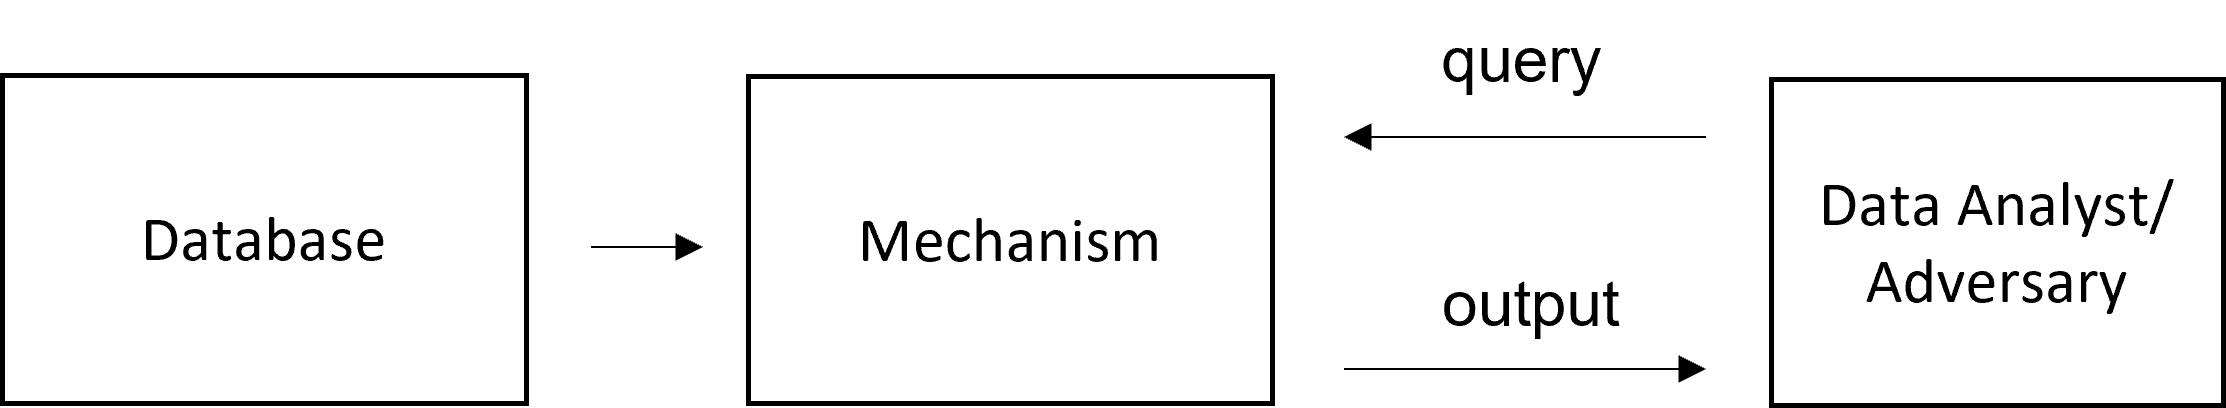
\includegraphics[width=\textwidth]{DP_setting}
    \centering
    \caption{DP setting.}
    \label{img:DPsetting}
\end{figure}
\FloatBarrier
% --------------------------------------------------------------------------

\begin{definition}[Neighboring Databases~\cite{dwork2014algorithmic}]
    Two databases $D_{0}$, $D_{1}\in \mathcal{X}^{n}$  are called neighboring if they differ in exact one entry. This is expressed as $D_{0}\sim D_{1}$.
\end{definition}

\begin{definition}[Differential Privacy~\cite{dwork2014algorithmic}]
    A privacy mechanism $M:\mathcal{X}^{n}\times \mathcal{Q}\rightarrow \mathcal{Y}$ is $\left( \varepsilon ,\delta \right)$-differential privacy if for any two neighboring databases $D_{1}$, $D_{1}\in \mathcal{X}^{n}$, and for all $T\subseteq \mathcal{Y}$, we have $\Pr \left[ M\left( D_{0}\right) \in T\right] \leq e^{\varepsilon}\cdot \Pr \left[ M\left( D_{1}\right) \in T\right] +\delta$ ,
    where the randomness is over the choices made by $M$.
    \label{def:DP}
\end{definition}

Roughly, the differential privacy implies that the distribution of $M$'s output for all neighboring databases is similar. $M$ is called $\varepsilon$-DP (or pure DP) when $\delta = 0$, and $\left(\varepsilon,\delta\right)$-DP (or approximate DP) when $\delta \neq 0$.

\begin{definition}[$L_{1}$ norm]
    The $L_{1}$ norm of a vector $\vec{X}=\left(x_1, x_2, \ldots,x_n \right)^{T}$ measures the sum of the magnitudes of the vectors $\vec{X}$ and is denoted by $\left\|\vec{X}\right\|_{1}=\sum ^{n}_{i=1}\left| x_{i}\right| $.
\end{definition}

\begin{definition}[$L_{2}$ norm]
    The $L_{2}$ norm of a vector $\vec{X}=\left(x_1, x_2, \ldots,x_n \right)^{T}$ measures the shortest distance of $\vec{X}$ to origin point and is denoted by $\left\|\vec{X}\right\|_{2}=\sqrt{\sum ^{n}_{i=1}x_{i}^{2}}$.
\end{definition}

\begin{definition}[$\ell_{t}$-sensitivity~\cite{dwork2014algorithmic}]
    The $\ell_{t}$-sensitivity of a query $f : \mathcal{X}^{n} \rightarrow \mathbb{R}^{k}$ is defined as $\Delta ^{\left(f\right)}_{t}=\max _{D_{0},D_{1}} \left\| f\left( D_{0}\right) -f\left( D_{1}\right) \right\| _{t}$, where $D_{0},D_{1}$ are neighboring databases and $t \in \left\{1,2\right\}$.
    \label{def:sensitivity}
\end{definition}
Recall the Differential Privacy Definition \autoref{def:DP} attempts to \textit{blur} the contribution of any individual in the database using the notion of neighboring databases. Therefore, the sensitivity is a natural quantity when considering differential privacy since it calculates the upper bound of how much $f$ can change when modifying a single entry.


\subsubsection{Motivating Example of Differential Privacy}
\label{subsubsec:motivatingexampleDP}
The previous example about randomized response \autoref{subsubsection:randomizedresponse} indicates that we need DP to solve the trade-off problem between learning useful statistics and preserving the individuals' privacy. In other words, the psychologist wants to find the fraction of students who have cheated in the exam while guaranteeing that no students suffer from privacy leakage by participating in the questionnaire.
To illustrate how DP solves such problems, we adapt the example from~\cite{simpleexplanDP}.
Consider a game as \autoref{prot:motivationexampleDP} shows,
\begin{itemize}
    \item A challenger implements a function $M$ that can calculate useful statistical information. An adversary proposes two data sets $D_{0}$ and $D_{1}$ that differ by only one entry and a test set $Q$.
    \item Given $M\left( D_{0}\right) $, $M\left( D_{1}\right) $ in a random order, the adversary aims to differentiate $D_{0}$ and $D_{1}$. If the adversary succeeds, privacy is violated.
    \item The challenger's goal is to choose $M$ such that $M\left( D_{0}\right) $ and $M\left( D_{1}\right) $ \textit{look} \textit{similar} to prevent them from being distinguished by the adversary.
    \item $M$ is called $\varepsilon$-differentially private iff: $\left| \frac{\Pr \left[ M\left( D_{0}\right) \in Q\right] }{\Pr \left[ M\left( D_{1}\right) \in Q \right] }\right|\leq e^{\varepsilon}$.
\end{itemize}

\begin{protocol}[tbh!]
    \centering
    \fbox{\pseudocode[space=none, syntaxhighlight=auto, addkeywords={input, output}]{%
    \textbf{Challenger $C$} \< \< \textbf{Adversary $A$} \\[0.1\baselineskip][\hline]
    \<\< \\[-0.5\baselineskip]
    \text{input: $M$} \< \< \text{input: $D_0$, $D_1$, $Q$ }\\
    \< \sendmessageleft{top={$D_0$, $D_1$}} \< \<  \\
    \text{$b \sample \bin$} \< \< \\
    \text{$M\left(D_{b}\right)$, $M\left(D_{1-b}\right)$} \< \< \\
    \< \sendmessageright{top={$M\left(D_{b}\right)$, $M\left(D_{1-b}\right)$}} \< \<  \\
    \< \< \text{$b^{\prime}=0$, if $M\left(D_{1-b}\right) \in Q $} \\
    \< \< \text{$b^{\prime}=1$, otherwise} \\
    \< \< \text{if $b==b^{\prime}$, $A$ wins.}
    }}
    \caption{A motivating example of differential privacy.}
    \label{prot:motivationexampleDP}
\end{protocol}
\FloatBarrier

Suppose the adversary $A$ has chosen two data sets:
\begin{itemize}
    \item $D_{0}=\left\{ 0, 0, 0,\ldots ,0\right\} $ ($100$ zeros)
    \item $D_{1}=\left\{ 1, 0, 0,\ldots ,0\right\} $ ($0$ one and $99$ zeroes).
\end{itemize}

The testing set $Q$ is an interval $\left[ T,1\right] $, where the threshold $T$ is chosen by the adversary. The threshold $T$ is chosen such that when the adversary has $T<M\left( D\right) < 1$, he knows $M$ has input $D=D_{1}$ (or $D=D_{0}$, when $0<M\left( S\right) \leq T$) .

\textbf{The Deterministic Case.}
Suppose the challenger wants to calculate the mean value of data sets and chooses $M\left( D\right) =mean\left( D \right) $. Since $M\left( D_{0}\right) =0$ and $M\left( D_{1}\right) =0.01$, the adversary can set $Q =\left[ 0.005,1\right] $ and identify precisely the database $D$ used in $M\left( D\right) $ every time they play the game. In \autoref{img:DPexamplenoisefree}, the green line represents the distribution of $M\left( D_{0}\right)$, whereas the orange line represents the distribution of $M\left( D_{1}\right)$ (plotted upside down for clarity). The vertical dotted line represents the threshold $T=0.005$ which separates $D_{0}$ and $D_{1}$ perfectly.

\begin{figure}[htbp]
    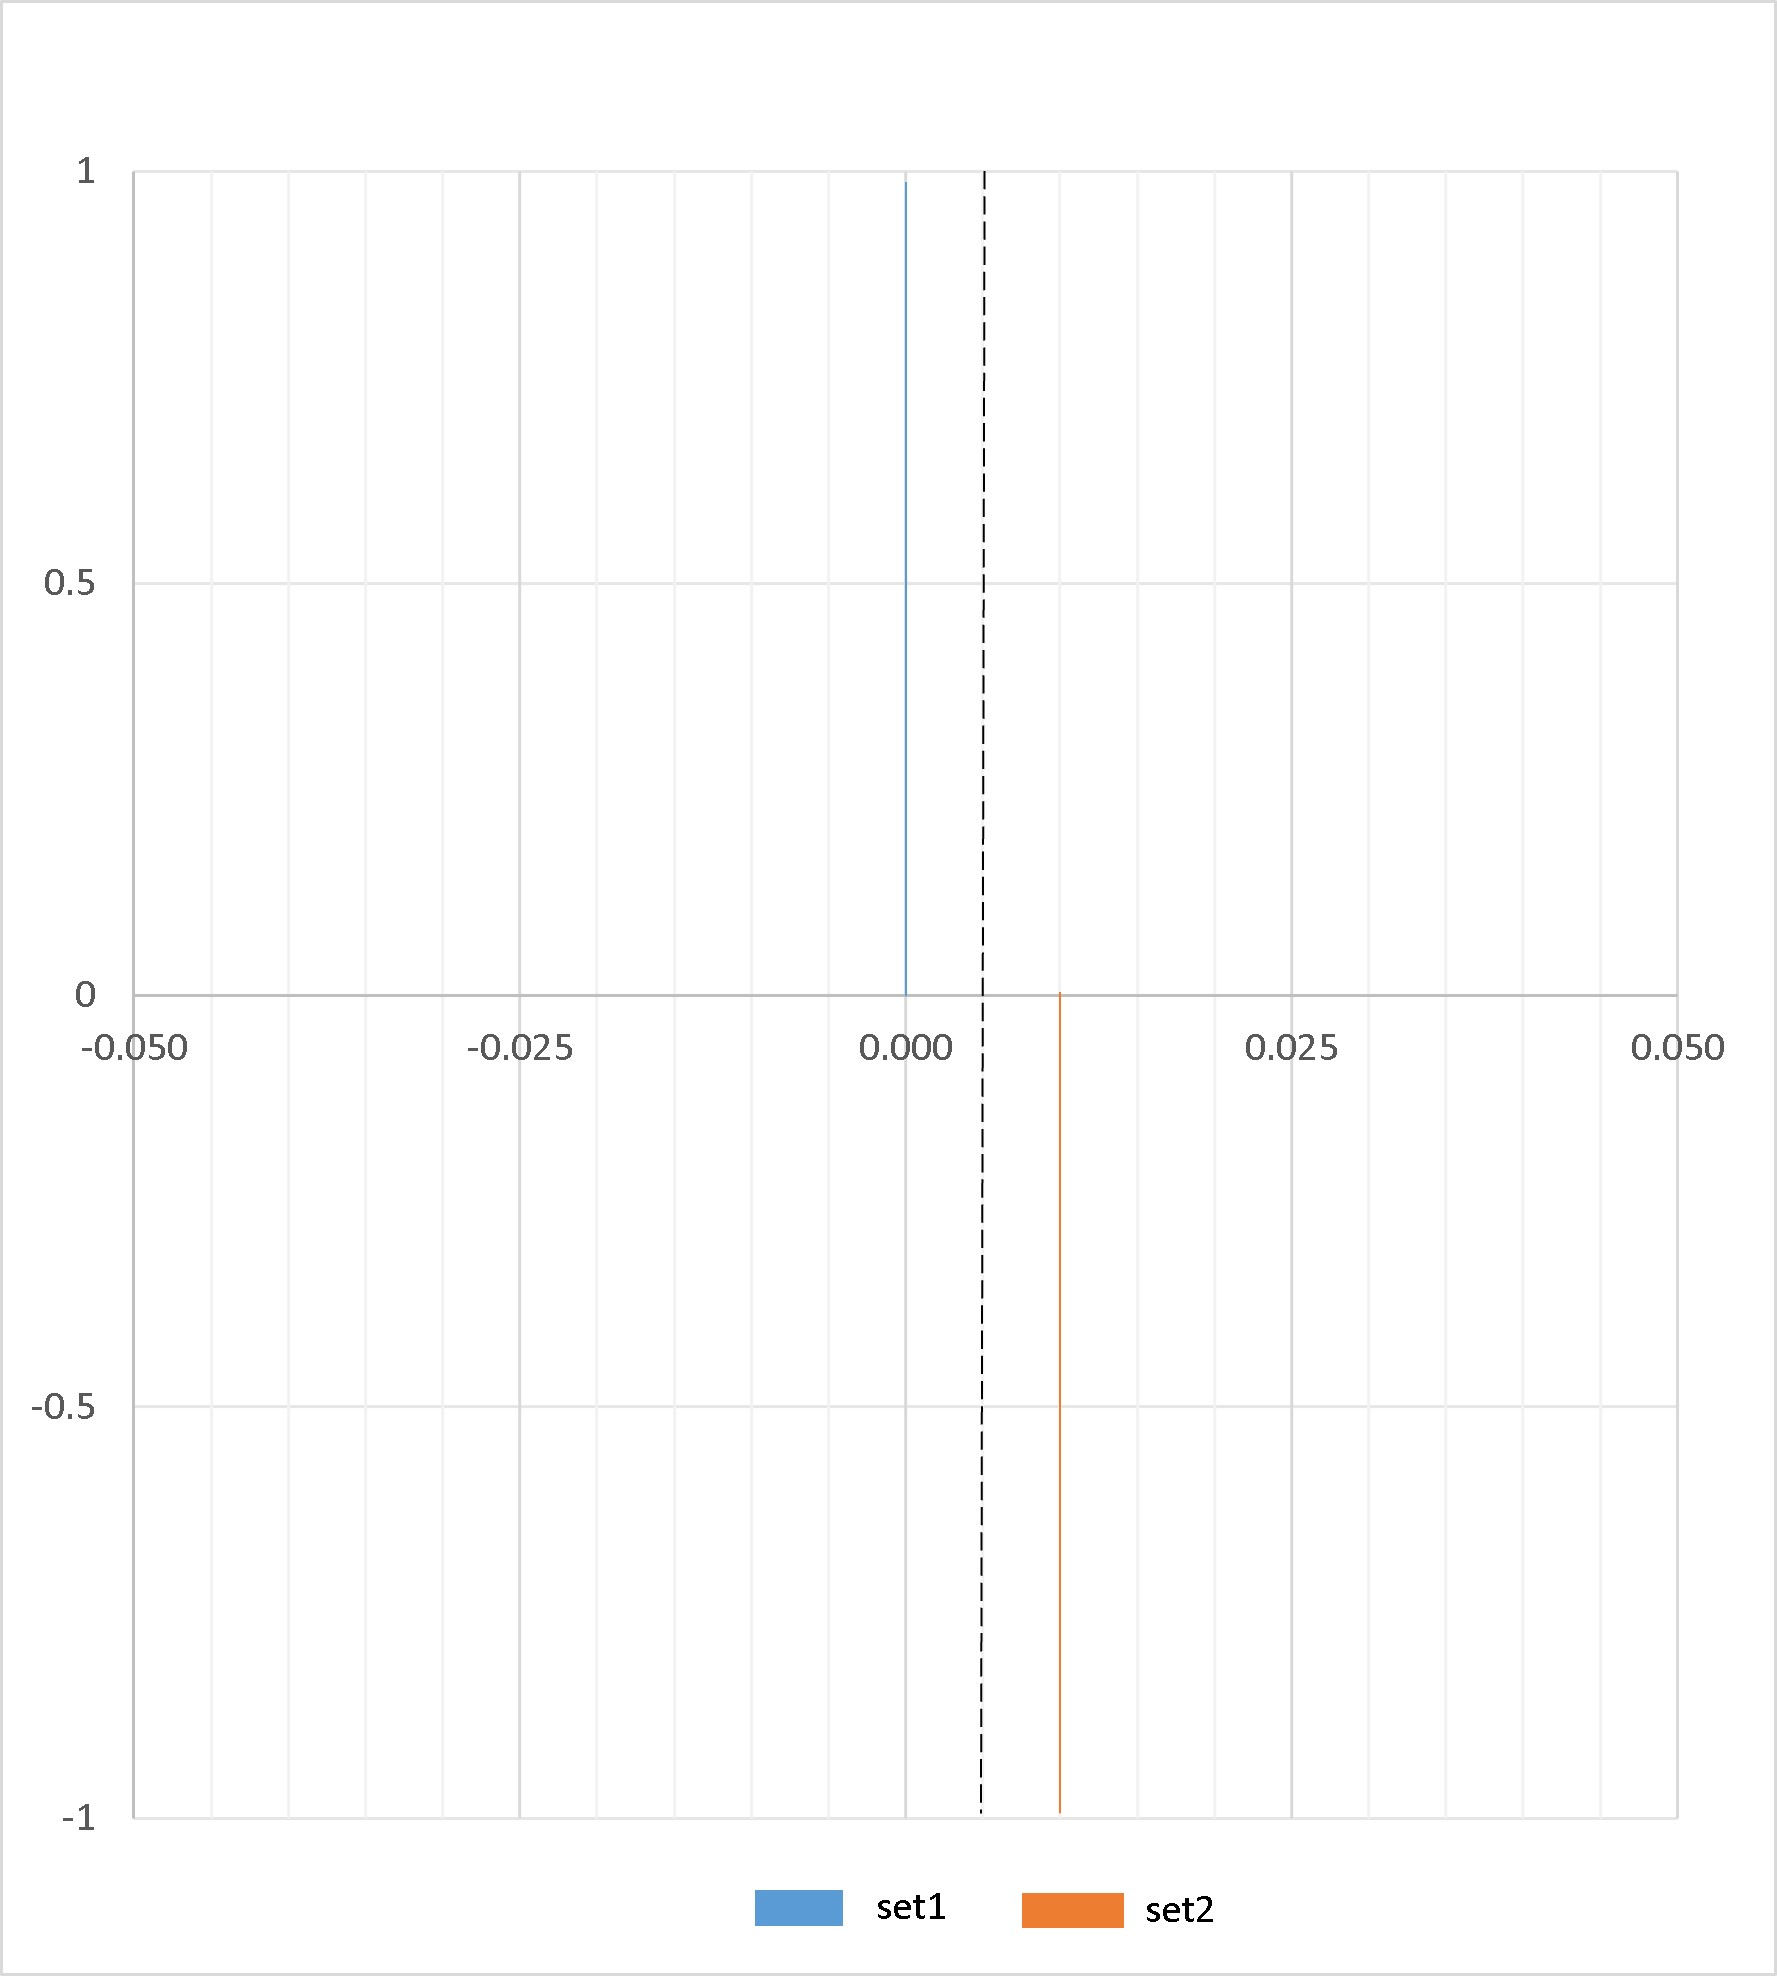
\includegraphics[width=10cm]{DPexamplenoisefree}
    \centering
    \caption{Deterministic algorithm (need reproduce).}
    \label{img:DPexamplenoisefree}
\end{figure}
\FloatBarrier

\textbf{The Indeterministic Case.}
The challenger needs to take some measures to \textit{blur} the difference between $M\left( D_{0}\right)$ and $M\left( D_{1}\right)$. Suppose the challenger decides to add Laplace noise $lap\sim Laplace\left(b=0.05\right)$ to the result of $M\left(D\right)$ as \autoref{img:DPexamplesmallnoise} shows. The shaded green region is the chance that $M\left( D_{0}\right)$ would return a value greater than the adversary's threshold $T$. In other words, the probability that the adversary would mistake $D_{0}$ for $D_{1}$. In contrast, the shaded orange area is the probability that the adversary identify $D$ as $D_{1}$. The challenger can decrease the adversary's probability of winning by adding more noise as \autoref{img:DPexamplelargenoise} shows, where the shaded green and orange areas are almost of the same size. Comparing $M\left( D\right)$ with $T$ is no longer reliable to distinguish $D_{0}$ and $D_{1}$. In fact, we have
$\varepsilon=\log \left( \frac{\text{green area}}{\text{orange area}}\right) $, where $\varepsilon$ expresses the degree of differential privacy and a smaller $\varepsilon$ guarantees a stronger privacy protection. Although the challenger can add more noise to decrease the adversary's success probability, the mean estimation accuracy is also decreased.


\TODO{need reproduce following figures}
\begin{figure}[htbp]
    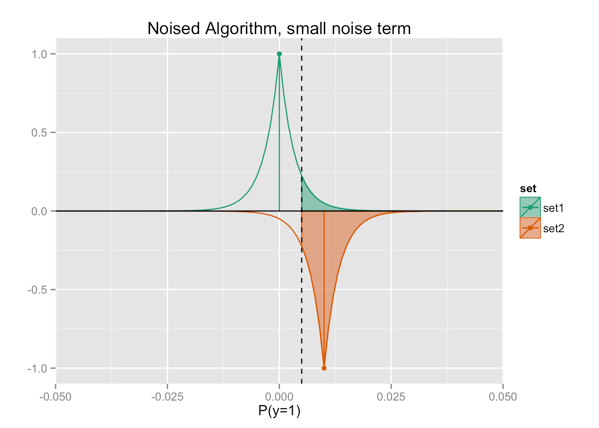
\includegraphics[width=10cm]{DPexamplesmallnoise}
    \centering
    \caption{Indeterministic algorithm with small noise ($b=0.005$) \TODO{(need reproduce)}.}
    \label{img:DPexamplesmallnoise}
\end{figure}
\FloatBarrier

\begin{figure}[htbp]
    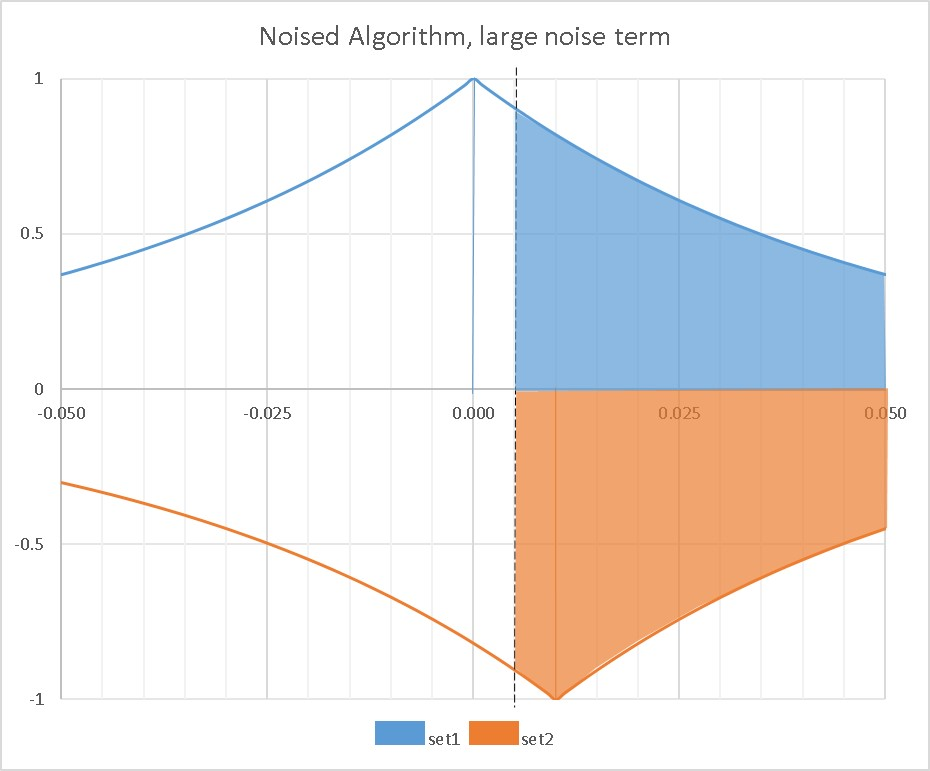
\includegraphics[width=10cm]{DPexamplelargenoise}
    \centering
    \caption{Indeterministic algorithm with large noise ($b=0.05$) \TODO{(need reproduce)}.}
    \label{img:DPexamplelargenoise}
\end{figure}
\FloatBarrier

\subsubsection{Properties of Differential Privacy}
% One reason for the success of differential privacy is its convenient properties which make it possible to deploy differentially private mechanisms in a modular fashion.

\paragraph{Post-Processing}
\begin{theorem} Let $M:\mathcal{X}^{n} \rightarrow \mathcal{Y}$ be $\left( \varepsilon ,\delta \right)$-DP mechanism, and let $F:\mathcal{Y}\rightarrow \mathcal{Z}$  be an arbitrary randomized mapping. Then $F\circ M$ is $\left( \varepsilon ,\delta=0 \right)$-DP~\cite{dwork2014algorithmic}.
\end{theorem}
The Post-Porcessing properties implies the fact that once a database is privatized, it is still differentially private after further processing.

\paragraph{Group Privacy}
\begin{theorem} Let $M:\mathcal{X}^{n} \rightarrow \mathcal{Y}$ be $\left( \varepsilon ,\delta \right)$-DP mechanism. For all $T\subseteq \mathcal{Y}$, we have $\Pr \left[ M\left(D_{0}\right) +T\right] \leq e^{k \varepsilon}\cdot \Pr \left[ M\left( D_{1}\right) \in T\right] +\delta$, where $D_{0}$, $D_{1}\in \mathcal{X}^{n}$ are two databases that differ in exactly $k$ entries~\cite{dwork2014algorithmic}.
\end{theorem}

Differential privacy can also be defined when considering two databases with more than one entry differences. The larger privacy decay rate $e^{k\varepsilon}$ implies a smaller $\varepsilon$, where \textit{more} noise are necessary to guarantee the same level of privacy.

\paragraph{Basic Composition}
\begin{theorem}
    Suppose $M=\left( M_{1}\ldots M_{k}\right)$  is a sequence of $\left( \varepsilon_{i} ,\delta_{i} \right)$-differentially private mechanisms, where $M_{i}$ is chosen sequentially and adaptively. Then $M$ is $\left(\sum_{i=1}^n\varepsilon_{i} ,\sum_{i=1}^n\delta_{i} \right)$-DP~\cite{dwork2014algorithmic}.
\end{theorem}

Basic Composition provides a way to evaluate the overall privacy when $k$ privacy mechanisms are applied on the same dataset and the results are released.

% \subsection{Comparison between Differential Private Mechanisms}
\subsubsection{Differentially Private Mechanisms}
\label{subsubsec:DPMechanisms}

Differential privacy is a formal framework to quantify the trade-off between privacy and the accuracy of query results. In this part, we introduce two common differentially private mechanisms.

\paragraph{$\varepsilon$-Differential Privacy}
\begin{definition}[Laplace Mechanism~\cite{dwork2014algorithmic}]\
    \label{def:laplaceMechanism}
    Let $f : \mathcal{X}^{n} \rightarrow \mathbb{R}^{k}$. The Laplace mechanism is defined as $M_{Lap}\left( X\right) =f\left( X\right) +\left( Y_{1},\ldots ,Y_{k}\right) $, where the $Y_{i}$ are independent Laplace random variables drawn from a Laplace distribution $Lap \left(  Y_{i}\,|\, b\right) =\frac{1}{2b}e^{\left( -\frac{\left  | Y_{i}\right|}{b}\right)} $ with $b=\frac{\Delta _{1}^{\left(f\right)}}{\varepsilon }$.
\end{definition}

\begin{theorem}
    Laplace Mechanism preservers $\varepsilon$-DP~\cite{dwork2014algorithmic}.
\end{theorem}



% \begin{proof}
%     Let $D_{0}$ and $D_{1}$ be any two neighbouring databases that differs in one entry. Let $\Pr_{D_{0}}\left(z\right) $ and $\Pr_{D_{1}}\left( z\right) $ be the probability density functions of $M\left( D_{0}\right) $ and $M\left( D_{1}\right) $ evaluated at a point $z \in \mathbb{R}^{k}$. To prove differential privacy, it necessary to show that the ratio $\frac{\Pr_{D_{0}}\left( z\right) }{\Pr_{D_{1}}\left( z\right) }$ is bounded by $\varepsilon$, for any arbitrary $z$ and neighboring $D_{0}$ and $D_{1}$ .

%     \begin{align*}
%         \frac{\Pr_{D_{0}}\left( z\right) }{\Pr_{D_{1}}\left( z\right) } & =\frac{ \prod _{i=1}^{k}\exp{\left( -\frac{ \varepsilon \left| f\left( D_{0}\right) _{i}-z_{i} \right|}{\Delta }\right) }}{\prod_{i=1}^{k}\exp{\left( -\frac{ \varepsilon \left| f\left( D_{1}\right) _{i}-z_{i} \right|}{\Delta }\right) } } \\
%                                                                         & =\prod_{i=1}^{k} \exp \left(-\frac{\varepsilon\left(\left|f(D_{0})_{i}-z_{i}\right|-\left|f(D_{1})_{i}-z_{i}\right|\right)}{\Delta}\right)                                                                                                    \\
%                                                                         & \leq \prod_{i=1}^{k} \exp \left(\frac{\varepsilon\left|f(D_{1})_{i}-f(D_{0})_{i}\right|}{\Delta}\right)                                                                                                                                       \\
%                                                                         & =\exp \left(\frac{\varepsilon \sum_{i=1}^{k}\left|f(D_{1})_{i}-f(D_{0})_{i}\right|}{\Delta}\right)                                                                                                                                            \\
%                                                                         & =\exp \left(\frac{\varepsilon\|f(D_{1})-f(D_{0})\|_{1}}{\Delta}\right)                                                                                                                                                                        \\
%                                                                         & \leq \exp (\varepsilon).                                                                                                                                                                                                                      \\
%     \end{align*}
% \end{proof}

% \begin{definition}[Privacy Loss~\cite{dwork2014algorithmic}]
%     Let $X$ and $Y$ be two random variables. The privacy loss random variable  $\mathcal{L}_{X||Y}$ is distributed by drawing $t \sim Y$ , and outputting $\ln ( \frac {\Pr \left[ X=t\right] )}{\Pr \left[ Y=t\right] )} $.
% \end{definition}

% The definition of \emph{Privacy Loss} relies on the assumption that the supports of $X$ and $Y$ are equal, where $supp\left(f\right)=\left\{x \in X: f\left(x\right) \neq 0\right\}$. Otherwise, the privacy loss is undefined since $\Pr\left\{Y=t\right\}=0$.

% From the definition of $\varepsilon$-DP, it is not difficult to see that $\varepsilon$-DP corresponds to $\left|\mathcal{L}_{D_{0}||D_{1}}\right|$ being bounded by $\varepsilon$ for all neighboring databases $D_{0}$, $D_{1}$. In other words, $\varepsilon$-DP says that the absolute value of the privacy loss random variable is bounded by $\varepsilon$ with probability 1.

\paragraph{$\left(\varepsilon,\delta\right)$-Differential Privacy}
$\varepsilon$-DP has strong privacy requirement which leads to adding too much noise and affecting the accuracy of the queries. We introduce an relaxation of $\varepsilon$-DP, $\left(\varepsilon,\delta\right)$-DP.

\begin{definition}[Gaussian Mechanism~\cite{dwork2014algorithmic}]
    Let $f : \mathcal{X}^{n} \rightarrow \mathbb{R}^{k}$. The Gaussian mechanism is defined as $M\left( X\right) =f\left( X\right) +\left( Y_{1},\ldots ,Y_{k}\right) $, where the $Y_{i}$ are independent Gaussian random variables drawn from distribution $\mathcal{N}  \left(  Y_{i}| \mu ,\sigma ^{2}\right) =\frac{1}{\sigma \sqrt{2\pi }}e^{-\frac{1}{2}\left( \frac{Y_{i}-\mu}{\sigma }\right) ^{2}}$ with  $\mu=0$, $\sigma ^{2}=2\ln \left( \frac{1.25}{\delta }\cdot \left( \frac{ \Delta _{2}^{\left(f\right)}) ^{2}}{\varepsilon ^{2}}\right) \right)$ .
    \label{def:gaussianMechanism}
\end{definition}

Gaussian mechanism is proved to satisfy $\left(\varepsilon,\delta\right)$-DP~\cite{dwork2014algorithmic}.



\subsubsection{Discussion about Differential Privacy}

\paragraph{Local and Central Differential Privacy}
Differential privacy is a definition that can be realized in many ways. Two common modes of DP are centralized differential privacy~\cite{dwork2014algorithmic} and local differential privacy~\cite{dinur2003revealing}.

In centralized DP, all data is stored centrally and managed by a trusted curator before the differentially private mechanism is applied. As \autoref{img:DPcentral} shows, the raw data from clients is first collected in a centralized database, then, the curator applies the privacy mechanism and answers the queries $f\left(x\right)$ with $f^{\prime}\left(x\right)$.
The local DP mode is, as \autoref{img:DPlocal} shows, where the clients first apply a privacy mechanism on their data, and send the perturbed data to the curator.
An advantage of local DP mode is that no trusted central curator is needed since the data is perturbed independently before sending to the curator. However, the disadvantage is that the collected data contains redundant noise and may decrease the utility.

\TODO{reproduce following figures}
\begin{figure}[htbp]
    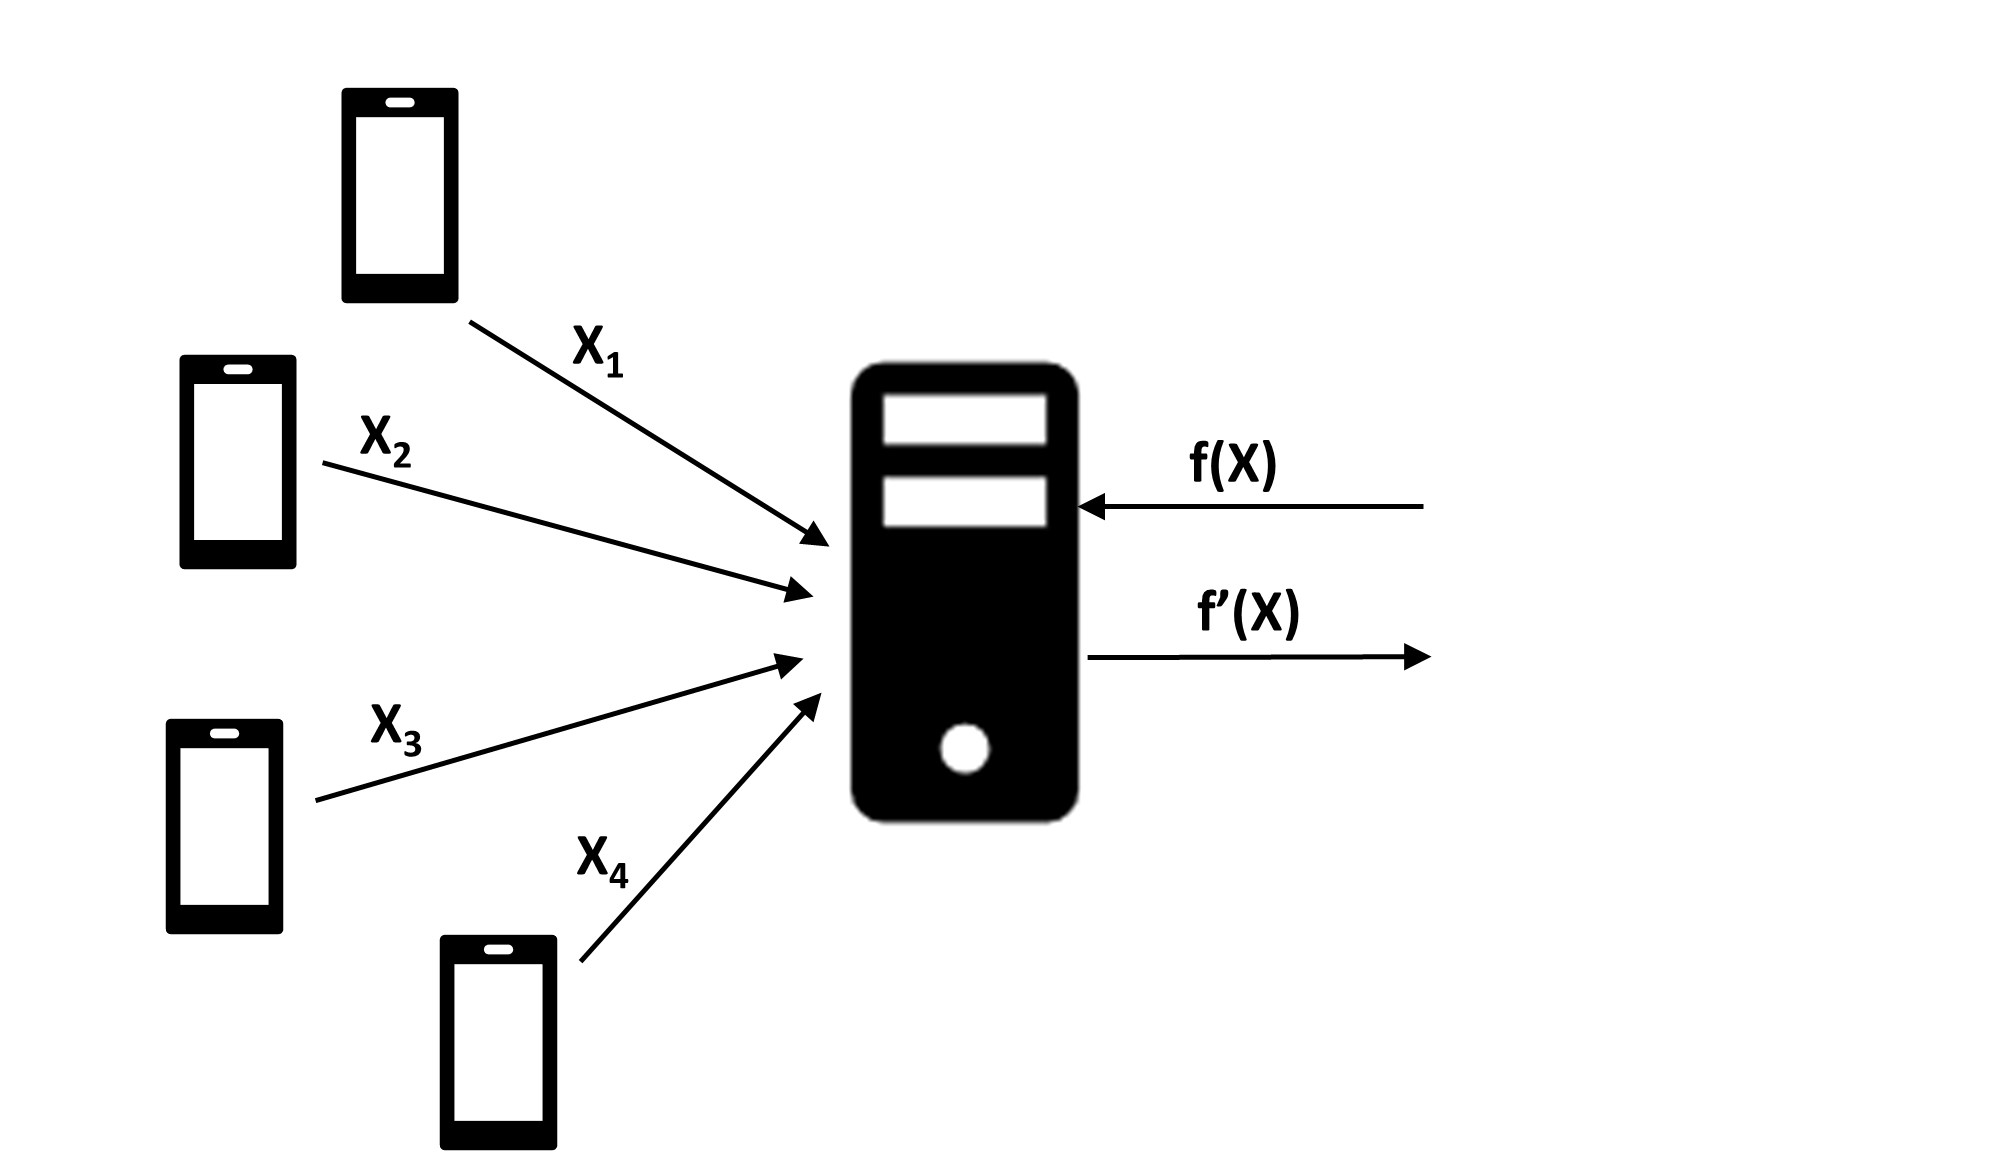
\includegraphics[width=10cm]{DPcentral}
    \centering
    \caption{Centralized DP mode (need reproduce).}
    \label{img:DPcentral}
\end{figure}
\FloatBarrier

\begin{figure}[htbp]
    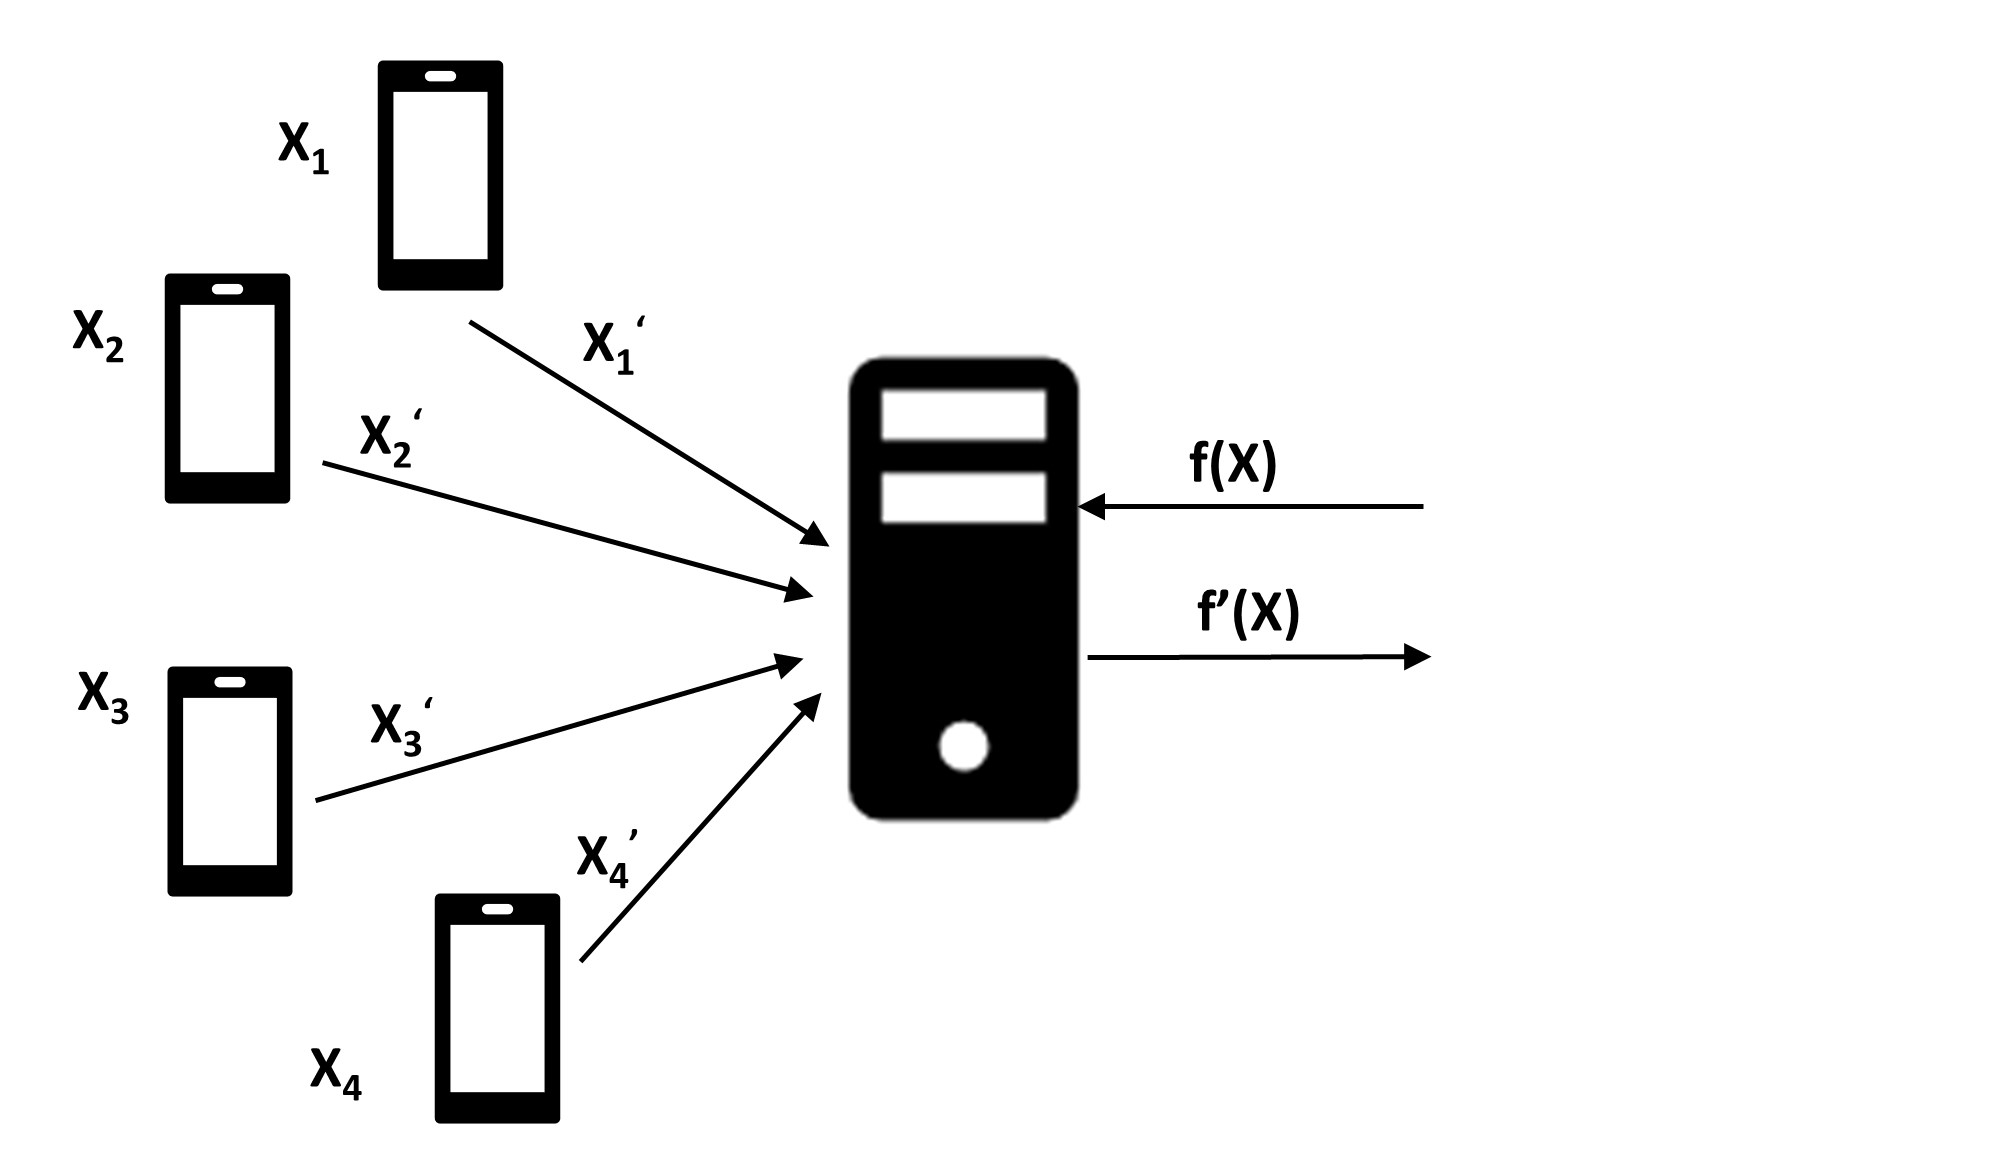
\includegraphics[width=10cm]{DPlocal}
    \centering
    \caption{Local DP mode (need reproduce).}
    \label{img:DPlocal}
\end{figure}
\FloatBarrier


\paragraph{Advantages of Differential Privacy}
From the example \autoref{subsubsec:motivatingexampleDP}, we found that DP can still protect privacy even if the adversary has the knowledge of the database. Generally speaking, DP ensures privacy protection by making no assumption about the adversary's auxiliary information (even when the adversary is the data provider) or computational strategy (regarding the complexity of modern cryptography)~\cite{vadhan2017complexity}. In addition, DP provides a quantitive theory about safely releasing data and maintaining certain level of accuracy.

\paragraph{Challenges of Differential Privacy}
\label{subsubsec:challengesOfDP}
DP provides a method to guarantee and quantify individual privacy at the theoretical level. However, it faces a series of practical challenges.

\textbf{Sensitivity Calculation}. For certain types of data, the sensitivity is not difficult to calculate. Take a database with human ages as an example, the ages should be bounded between $0$ and $150$ (longest human lifespan is $122$ years and $164$ days according to~\cite{whitney_1997}). However, the data with an unbounded value range brings great challenges. A common solution is to roughly estimate the value range and limit the data within that range. For example, if the value range estimation is $\left[ a,b\right] $, then all values smaller than $a$ are replaced by $a$ and all values bigger than $b$ are replaced by $b$. Finally, the sensitivity of query function that outputs ages is ${b- a}$. If value range $\left[ a,b\right] $ is chosen too wide, the utility is potentially destroyed because of the large magnitude of the noise. If the value range $\left[ a,b\right] $ is chosen too narrow, the utility is also potentially decreased because too many values beyond $\left[ a,b\right] $ are truncated.

\textbf{Implementation of DP Mechanisms}. The theory of DP is built upon the real number arithmetic. The practical implementation of differentially private mechanisms relies on floating-point or fixed-point arithmetic only provides an approximation of the mathematical abstractions. Mironov~\cite{mironov2012significance} showed that the irregularities of floating-point implementations and porouse distribution of the Laplace mechanism with textbook sampling algorithm lead to the breach of differential privacy. Further, Gazeau et al.~\cite{gazeau2016preserving} proved that any differentially private mechanism that perturbs data by adding noise with a finite precision can resulting secret disclosure regardless of the actual implementation.

% -------------------------------------------------------------


% Similar to $\varepsilon$-DP, $\left(\varepsilon,\delta\right)$-DP can also be interpreted regarding privacy loss: the absolute value of the privacy loss random variable is bounded by $\varepsilon$ with probability $1 - \delta$~\cite[Lemma 3.17]{dwork2014algorithmic}. In other words, with probability $ \delta$, the privacy of databases is breached.
